%{{{ Nastaveni
%%%%%%%%%%%%%%%%%%%%%%%%%%%%%%%%%%%%%%%%%%
%%%                                    %%%
%%% Šablona bakalářské práce na MFF UK %%%
%%%                                    %%%
%%% (c) František Štrupl, 2005         %%%
%%%                                    %%%
%%%%%%%%%%%%%%%%%%%%%%%%%%%%%%%%%%%%%%%%%%

%%% POZOR: Úprava bakalářské práce je závislá rovněž na volbě jednostranného resp. oboustranného tisku.
%%%        Bližši informace naleznete v dokumentu Úprava bakalářské práce, který se nalézá na adrese:
%%%        http://www.mff.cuni.cz/studium/obecne/bplayout/pok12mo4.pdf

\documentclass[12pt,notitlepage]{report}
%\pagestyle{headings}
\pagestyle{plain}

\frenchspacing % aktivuje použití některých českých typografických pravidel

\usepackage[utf8]{inputenc} % nastavuje použité kódování, uživatelé Windows zamění latin2 za cp1250
\usepackage[czech]{babel}
\usepackage{a4wide} % nastavuje standardní evropský formát stránek A4
%\usepackage{index} % nutno použít v případě tvorby rejstříku balíčkem makeindex
%\usepackage{fancybox} % umožňuje pokročilé rámečkování :-)
\usepackage[pdftex]{graphicx} % nezbytné pro standardní vkládání obrázků do dokumentu
\usepackage{hyperref}
\usepackage{epstopdf}
\usepackage{url}
\usepackage{minted}
\usepackage{caption}

\usepackage[left=4cm]{geometry} % nastavení dané velikosti okrajů

\renewcommand\listingscaption{Zdrojový kód}
\newminted[pyc]{python}{linenos=true, frame=lines}

\newenvironment{mylisting}{}{}

\newcommand{\code}[1]{\texttt{\small #1}}
\newcommand{\method}[1]{\vskip.5cm \texttt{\small #1}}

\newenvironment{popis}%
{\begin{list}{}%
         {\setlength{\leftmargin}{0.5cm}\setlength{\topsep}{1pt}
          \setlength{\itemsep}{0.1cm} \setlength{\parsep}{0.2cm}}%
         \item[]%
}
{\end{list}}

%\newindex{default}{idx}{ind}{Rejstřík} % zavádí rejstřík v případě použití balíku index

\title{Řízení robota e-Puck v Pythonu}   % tyto dvě položky jsou zde v podstatě formálně, ve skutečnosti nejsou nikde
\author{David Marek} % dále v dokumentu použity

%\date{}

%}}}
\begin{document}
%{{{ Titulka a dalsi stranky pred textem
%\csprimeson % zapne jednoduché psaní českých uvozovek pomocí klasických znaků, ale potom pozor
             % na originální apostrofy, které budou chybně interpretovány!!!

%%% Následuje první, úvodní, strana bakalářské práce. Jednotlivé položky nahraďte dle vlastních
%%% údajů. Změnit podle konkrétní délky jednotlivých položek můžete i zalomení řádků.
\begin{titlepage}
\begin{center}
\ \\

\vspace{15mm}

\large
Univerzita Karlova v Praze\\
Matematicko-fyzikální fakulta\\

\vspace{5mm}

{\Large\bf BAKALÁŘSKÁ PRÁCE}

\vspace{10mm}

%%% Aby vložní loga vše správně fungovalo, je třeba mít soubor logo.eps nahraný v pracovním adresáři,
%%% tj. v adresáři, kde se nachází překládaný zdrojový soubor. Soubor logo.eps je možné získat např.
%%% na adrese: http://www.mff.cuni.cz/fakulta/symboly/logo.eps

\includegraphics[scale=0.3]{logo.eps}

\vspace{15mm}

%\normalsize
{\Large David Marek}\\ % doplňte vaše jméno
\vspace{5mm}
{\Large\bf Řízení robota e-puck v Pythonu}\\ % doplňte název práce
\vspace{5mm}
Kabinet software a výuky informatiky\\ % doplňte název katedry či ústavu
\end{center}
\vspace{15mm}

\large
\noindent Vedoucí bakalářské práce: RNDr. František Mráz, CSc. % doplňte odpovídající údaje
%%% další řádek můžete ve většině případů (tj. pokud údaje uvedené výše nejsou příliš dlouhé) zrušit
\vspace{1mm}

\noindent Studijní program: Obecná Informatika
%\noindent Studijní program: název studijního programu, název studijního % doplňte odpovídající údaje
%%% další řádek můžete ve většině případů (tj. pokud údaje uvedené výše nejsou příliš dlouhé) zrušit
%\hskip20mm oboru (směru),  příp. název studijního plánu

\vspace{20mm}

\begin{center}
2010 % doplňte rok vzniku vaší bakalářské práce
\end{center}

\end{titlepage} % zde končí úvodní strana

\normalsize % nastavení normální velikosti fontu
\setcounter{page}{2} % nastavení číslování stránek
\ \vspace{10mm}

\noindent Na tomto místě mohou být napsána případná poděkování (vedoucímu práce, konzultantovi, tomu, kdo půjčil software, literaturu, poskytl data apod.). % doplňte vlastní text

\vspace{\fill} % nastavuje dynamické umístění následujícího textu do spodní části stránky
\noindent Prohlašuji, že jsem svou bakalářskou práci napsal samostatně a výhradně s použitím citovaných pramenů. Souhlasím se zapůjčováním práce a jejím zveřejňováním.

\bigskip
\noindent V Praze dne \hspace{\fill}David Marek\\ % doplňte patřičné datum, jméno a příjmení

%%%   Výtisk pak na tomto míste nezapomeňte PODEPSAT!
%%%                                         *********

\tableofcontents % vkládá automaticky generovaný obsah dokumentu

\newpage % přechod na novou stránku

%%% Následuje strana s abstrakty. Doplňte vlastní údaje.
\noindent
Název práce: Řízení robota e-puck v Pythonu\\
Autor: David Marek\\
Katedra (ústav): Kabinet software a výuky informatiky\\
Vedoucí bakalářské práce: RNDr. František Mráz, CSc.\\
E-mail vedoucího: mraz@ksvi.mff.cuni.cz\\

\noindent Abstrakt:  V předložené práci studujeme ... Uvede se abstrakt v rozsahu 80 až 200 slov. Lorem ipsum dolor sit amet, consectetuer adipiscing elit. Ut sit amet sem. Mauris nec turpis ac sem mollis pretium. Suspendisse neque massa, suscipit id, dictum in, porta at, quam. Nunc suscipit, pede vel elementum pretium, nisl urna sodales velit, sit amet auctor elit quam id tellus. Nullam sollicitudin. Donec hendrerit. Aliquam ac nibh. Vivamus mi. Sed felis. Proin pretium elit in neque. Pellentesque at turpis. Maecenas convallis. Vestibulum id lectus. Fusce dictum augue ut nibh. Etiam non urna nec mi mattis volutpat. Curabitur in tortor at magna nonummy gravida. Mauris turpis quam, volutpat quis, porttitor ut, condimentum sit amet, felis.\\

\noindent Klíčová slova: klíčová slova (3 až 5)

\vspace{10mm}

\noindent
Title: Název bakalářské práce v angličtině\\
Author: Jméno autora\\
Department: Název katedry či ústavu v angličtině\\
Supervisor: Jméno s tituly jako v české verzi, event. pracoviště\\
Supervisor's e-mail address: e-mailová adresa vedoucího\\

\noindent Abstract: In the present work we study ... Uvede se anglický abstrakt v rozsahu 80 až 200 slov. \\

\noindent Keywords: klíčová slova (3 až 5) v angličtině

\newpage

%}}}
\chapter{Úvod} %{{{

    \section{Záměr práce}

    Cílem této práce je vytvořit uživatelsky přívětivou a intuitivní knihovnu v
    programovacím jazyku Python, kterou budou moci použít studenti pro ovládání
    e-puck robota. Tato knihovna jim umožní ovládat všechny části robota z PC
    přes Bluetooth spojení. Díky tomu budou moci využít výkonu svého počítače
    pro vytváření programů, které by nebylo možné uskutečnit v robotovi kvůli
    omezením jeho mikrokontroleru.

    Většina knihoven pro ovládání robota umožňuje pouze synchronní komunikaci.
    Součástí této práce ovšem bude i možnost provádět příkazy asynchronně. Z
    toho důvodu je součástí práce i firmware robota, který umožní uživateli
    nejen využít asynchronní komunikaci, ale také zlepšení spolehlivosti
    přenosu. Dále bude provedeno několik úprav, které rozšíří možnosti ovládání
    robota (např. signalizace vybité baterie, anebo možnost získat hodnoty z
    mikrofonu).

    Práce by měla sloužit pro potřeby studentů zajímajících se o vývoj
    programů pro ovládání e-puck robota. Pro seznámení s knihovnou a možnostmi
    robota tedy bude součástí knihovny i několik ukázkových programů. Umožní
    čitateli napsat si svůj vlastní program velmi rychle, s využitím konstrukcí
    ukázaných v příkladech, anebo pouze inspirováním.

    Knihovna bude mít velmi jednoduché rozhraní, díky kterému bude možné
    ovládat robota bez složité inicializace, kupříkladu i interaktivně z
    interpretu Pythonu. Také bude možné knihovnu používat ve spolupráci s
    externími knihovnami. Výsledkem bude např. jednoduché vytváření grafických
    aplikací, anebo zpracování obrázků z kamery pomocí externích nástrojů.

    \section{Přehled kapitol}

    \subsection{Teoretická část}
    V první části práce jsou představeny podklady a teoretické informace
    vázající se k tématu. Po přečtení této části by měly být jasné všechny
    pojmy a čitatel by měl mít dostatečné informace o problematice programování
    robota pro napsání vlastního programu.

    V kapitole \ref{e-puck robot} je představen e-puck robot. Je zde popsán
    účel robota, okolnosti jeho vzniku a také všechny senzory a akční členy.
    Také se zde uživatel dozví jaké jsou možnosti programování robota.

    Při vzdáleném ovládání robota je velmi důležitá komunikace mezi ním a
    počítačem, na kterém je spuštěn ovládací program. Kapitola \ref{sync/async}
    představuje rozdíly mezi komunikací synchronní a asynchronní. Vysvětluje
    jaké jsou výhody a nevýhody obou řešení a jak se s nimi e-puck knihovna
    vyrovnává.

    V kapitole \ref{existujici prace} čitatel zjistí, že tato práce není
    jediným pokusem o knihovnu pro ovládání robota. Bude představeno několik
    programů, které slouží k ovládání anebo simulaci robota. Také budou
    představeny knihy, které mohou sloužit pro rozšíření informací uvedených v
    této práci, anebo jako zdroj inspirace pro kontrolní programy.

    Nakonec bude představena specifikace knihovny (část \ref{specifikace}).
    Čitatel se dozví jakými problémy trpěl původní firmware a jaké jsou nutné
    změny, které bylo třeba vykonat. Dále jsou zde uvedena všechna vylepšení,
    díky kterým se knihovna snaží soupeřit s konkurencí.

    \subsection{Praktická část}
    V druhé části práce bude představena implementace knihovny. Bude
    vysvětleno, jak byly použity mechanismy představené v teoretické části,
    díky kterým může být komunikace asynchronní. Také budou představeny
    přídavky ke standardním možnostem robota.

    V kapitole \ref{btcom} je představen firmware BTcom, jak funguje posílání
    příkazů robotovi a také zde jsou popsány všechny změny, které byly vykonány
    na firmware robota.

    Synchronní komunikace je předvedena v části \ref{btcom:sync} i s krátkou
    ukázkou jak zasílat příkazy.

    Asynchronní komunikace je druhým způsobem jak robotovi zasílat příkazy, je
    o poznání složitější než synchronní komunikace a tedy je jí věnováno více
    místa v části \ref{async-impl}. Čitatel se dozví co vše se děje na pozadí
    při posílání asynchronních zpráv.

    Jak funguje samotné ovládání robota je popsáno v části \ref{controller}.
    Ovládání se liší podle komunikace. Při synchronní je transparentní a
    jednoduché, při asynchronní je na druhou stranu spolehlivé, i když přináší
    do komunikace jednu vrstvu navíc.

    \subsection{Příklady}

    V části \ref{dokumentace} je návod pro práci s e-puck robotem. Ten začíná u
    připojení robota k počítači a končí zasíláním příkazů. Také je zde uveden
    ukázkový program a následně rozebrán řádek po řádku.

    Následují příklady kontrolních programů v kapitole \ref{priklady}. Jde o
    příklad ovládání robota a vyhýbání se překážkám (Braitenberg vehicle v
    sekci \ref{braitenberg vehicle}), dále možnost změny programu pomocí
    přepínače na robotovi (příklad \ref{LED}) a nakonec využití kamery a
    externích knihoven pro detekci obličejů (příklad \ref{face detection}).

    \subsection{Přílohy}

    Nakonec už následují jen přílohy. V příloze \ref{dokumentace api} čitatel
    nalezne popis všech metod, které slouží pro ovládání robota. Jedná se o
    popis všech příkazů, které je možné robotovi poslat.

%}}}
\chapter{Teorie} %{{{

    V této části bych rád uvedl všechny základní součásti, na kterých má práce
    stojí a také bych se rád zmínil o způsobech jak se řeší ovládání robota
    jinde. Nejprve je nutné zjistit jaké vlastnosti má robot e-puck, abychom
    pak dále mohli posoudit do jaké míry využíváme jeho předností a také
    zhodnotit využitelnost práce v praxi. Popis e-puck robota je v sekci
    \ref{e-puck robot}. Dále je potřeba zmínit jakými způsoby může probíhat
    komunikace, jaká úskalí přináší oddělení kontrolního programu od hardware a
    jak se dají mírnit rizika z tohoto plynoucí, tím se zabývá sekce
    \ref{sync/async}.

    \section{E-puck robot}
    \label{e-puck robot}
    E-puck je miniaturní robot vytvořený pro výukové účely na akademické
    úrovni. Vytvořen byl v Ecole Polytechnique Fédérale de Laussanne. Celý
    projekt je založen na konceptu otevřeného hardware, což znamená, že všechny
    dokumenty a schémata jsou dostupná pod svobodnou licencí umožňující
    komukoli využívat e-puck robota na maximum a vyvíjet pro něj ať už
    software, anebo např. hardwarové nádstavby.

    \begin{listing}
        \begin{center}
            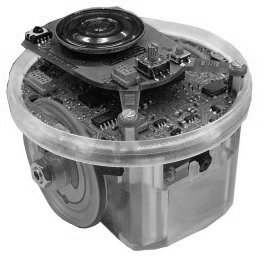
\includegraphics[scale=0.5]{e-puck.jpg}
            \caption{E-puck robot}
        \end{center}
    \end{listing}

    E-puck robot byl vytvořen s několika kritérii \cite{bonani}:
    \begin{itemize}
        \item Stolní velikost -- možnost experimentovat s robotem přímo u
        počítače je velmi výhodná pro studenty. Pokud se za optimální velikost
        pracovní plochy považuje 10-ti násobek velikosti robota, tak e-puck se
        svým průměrem 75mm je ideální pro použití na stole.

        \item Široké spektrum použití -- robota je možné použít nejen pro výuku
        robotiky, ale také například pro výuku zpracování obrazu nebo zvuku,
        programování vestavěných systémů, automatizace atd. Toho je docíleno
        velkým spektrem sensorů.

        \item Uživatelská přívětivost -- při vytváření rozhraní by vždy měl být
        kladen důraz na jednoduchost. Rozhraní by mělo být intuitivní a
        důkladně zdokumentované, aby se zrychlil proces učení.

        \item Možnost vzdáleného ovládání -- robot v sobě obsahuje Bluetooth
        modul, který se pro něj chová jako sériové zařízení, přes které dokáže
        komunikovat s počítačem.
    \end{itemize}

    Součástí robota je velká škála sensorů a akčních členů. Srdcem robota je
    mikrokontroler s obvodem dsPIC. Skládá se z 16bitového procesoru a jednotky
    pro zpracování signálu. Procesor má frekvenci 64 MHz, 8 kB RAM a 144 kB
    flash paměti. Robot obsahuje následující sensory:

    \begin{itemize}
        \item Infračervené sensory -- po obvodu robota je 8 IR sensorů. Měří
        buď vzdálenost od překážek, anebo intenzitu okolního světla. Jedná se o
        základní sensory využívané pro pohyb mezi překážkami.

        \item Akcelerometr -- 3D akcelerometr slouží k získání vektoru
        zrychlení robota. Může být použit pro spoustu experimentů (měření
        náklonu, zrychlení, detekce nárazu, pádu, \ldots).

        \item 3 mikrofony -- více mikrofonů slouží k triangulaci zdroje zvuku,
        velikost dat získaných z mikrofonů je ovšem na kapacity robota příliš a
        proto je nutné použít jednotku pro zpracování signálu (DSP).

        \item Barevná kamera -- v přední části robota je kamera s rozlišením
        640x480, bohužel kvůli paměťovým omezením robota je možné získat pouze
        část obrazu. I tak je ale možné ji použít pro experimenty s počítačovým
        viděním.
    \end{itemize}

    Samotné sensory by samozřejmě byly bez užitku, kdyby robot neměl žádné
    akční členy. Studenti mohou využít následujících komponent:
    \begin{itemize}
        \item 2 krokové motory -- slouží pro pohyb robota, mají rozlišení 1000
        kroků za jedno otočení kola.

        \item Reproduktor -- ve spojení s mikrofony může sloužit pro dorozumívání s
        jinými roboty, také jde o výhodný způsob interakce s uživatelem.

        \item 8 LED -- diody jsou rozmístěné po obvodu robota. Slouží jako
        vizuální rozhraní pro uživatele, anebo pro jiného robota.

        \item Zelená dioda uvnitř robota -- hlavním jejím posláním je zkrášlit
        robota, ale také může být použita pro interakci s jinými objekty.

        \item Přední dioda u kamery -- tato LED nevytváří rozptýlené světlo,
        ale paprsek, který je možné použít s kamerou pro odhadování vzdálenosti
        k vzdálenějším překážkám.
    \end{itemize}

    Ovládání e-puck robota je možné řešit několika způsoby. V první řadě
    existuje kompatibilní GCC kompilátor, takže je možné psát řídící program,
    který bude vykonáván přímo uvnitř robota, v programovacím jazyku C. Výrobce
    navíc dodává knihovnu s intuitivním rozhraním pro ovládání všech součástí.
    Tento přístup má ovšem několik nevýhod. Cyklus vývoje programu je pomalý,
    kvůli každé změně v programu je třeba spustit kompilaci na počítači, dále
    nahrát program do robota a teprve pak je možné změnu vyzkoušet. Dalším
    problémem je výkon robota, který nemusí stačit pro složitější výpočty.

    Lepším způsobem se tedy zdá využívat program v robotovi pouze pro
    vykonávání příkazů, které jsou naplánovány v počítači. To je přístup,
    kterým se zabývá tato práce. Získáme tím jednu obrovskou výhodu, kterou je
    výpočetní síla stolního počítače, na druhou stranu s ní ovšem musíme
    přijmout i břímě problémů s komunikací.

    \section{Synchronní / asynchronní komunikace}
    \label{sync/async}

    Pojem komunikace ve světě počítačů označuje předávání dat mezi dvěma
    programy nebo zařízeními. Příkladem může být komunikace mezi webovým
    prohlížečem a http serverem při stahování stránky, počítačem a tiskárnou
    při tisku, atd. Průběh komunikace je vždy velmi podobný, jedna strana pošle
    zprávu obsahující požadavek, druhá strana zprávu přijme a zpracuje. Pokud
    ke zpracování potřebuje další informace, pošle odesílateli jako odpověď
    žádost o jejich dodání a tak si zúčastněné strany vymění role a situace se
    opakuje.

    Přenos zprávy ovšem může zabrat netriviálně mnoho času a tak je tu problém,
    co bude dělat odesílatel zprávy, zatímco čeká na odpověď. Tady dochází k
    rozdělení na synchronní (nebo také blokující) a asynchronní (neblokující)
    komunikaci. Popisem synchronní komunikace se zabývá sekce \ref{sync},
    popisem asynchronní komunikace sekce \ref{async}. A nakonec je v sekci
    \ref{comm-epuck} popsáno jak byly tyto principy uplatněny v praxi.

    \subsection{Synchronní komunikace}
    \label{sync}

    Při synchronní komunikaci program po odeslání zprávy pozastaví vykonávání
    dalších instrukcí a čeká dokud nedostane odpověď. Tento přístup je velmi
    jednoduchý na implementaci (většinou se jedná o zavolání metody, která
    neskončí, dokud neobdrží zprávu), není problém s nekonzistencí dat (než
    bude program pokračovat v činnosti, obdrží všechny informace).

    Překážkou pro synchronní komunikaci jsou ovšem ztráty zpráv při přenosu.
    Může dojít k chybě při přenosu dat a ke ztrátě odeslané zprávy, anebo
    příchozí odpovědi. Stejně tak se může stát, že adresát zprávy na ni nijak
    neodpověděl. V takovýchto případech lehce dojde k tzv. dead-locku, kdy bude
    odesílatel čekat na zprávu, která nikdy nepřijde a tak nebude moci
    pokračovat v dalších výpočtech.

    Dochází také k mrhání procesorovým časem, čas strávený čekáním na odpověď
    by mohl být smysluplně využit. Typickým příkladem je grafické rozhraní, kde
    je potřeba zaručit interakci a nereagování na akce uživatele je ukazatelem
    špatně napsané aplikace. Ale nemusí jít jen o složité aplikace s grafickým
    rozhraním, čas strávený čekáním lze využít například pro zpracování
    již přijatých dat a díky tomu zvýšit jejich průtok.

    \subsection{Asynchronní komunikace}
    \label{async}

    Pokud je po programu požadována interaktivita, anebo komunikace není jeho
    jediným úkolem a musí zvládat například obsluhovat více blokovaných
    spojení, tak synchronní komunikace přestává stačit.

    Asynchronní komunikace řeší některé problémy komunikace synchronní. Po
    odeslání zprávy program pokračuje ve vykonávání instrukcí, nečeká na
    odpověď. Může si ale kdykoli zkontrolovat, zda-li už nepřišla odpověď a pak
    ji teprve načíst a zpracovat. Speciálním případem je komunikace řízená
    událostmi (event-driven), kdy je pro zpracování události přijetí zprávy
    určena funkce, která je automaticky spuštěna, bez přímé intervence
    programátora.

    Asynchronní komunikace velmi zjednodušuje vyřešení problémů se ztrátou
    zpráv. Protože program se musí sám podívat jestli nepřišla odpověď, tak si
    také může pamatovat, kdy byla odeslána zpráva a pokud odpověď nedorazí do
    určitého času, tak zprávu prohlásí za ztracenou a může se pokusit ji poslat
    znova.

    I asynchronní komunikace má své problémy. Odpovědi na zprávy nemusí přijít
    ve stejném pořadí, v jakém byly odeslány. Tento problém musí řešit
    například protokol TCP/IP. Řešením je zprávy posílat s pořadovým číslem a
    toto číslo přidat i k odpovědi. Pak je velmi snadné příchozí zprávy seřadit
    podle pořadí, v jakém jsou požadovány.

    \subsection{Komunikace v e-puck knihovně}
    \label{comm-epuck}

    V této práci je uživateli knihovny dána možnost vybrat si mezi komunikací
    synchronní a asynchronní. Synchronní komunikace je určena pro rychlé
    prototypování a zkoušení ovládání robota. Uživatel bude zadávat příkazy a
    dívat se, jak na ně robot reaguje. Tady je výhodná transparentnost
    synchronního přístupu. Naopak pro psaní kontrolních programů je větší důraz
    kladen na spolehlivost. Knihovna zajistí, že příkaz opravdu dojde, v
    nejhorším případě upozorní uživatele na skutečnost, že robot je
    neovladatelný (může se stát třeba pokud mu dochází baterie).

    Máme zde tu výhodu, že e-puck robot vždy pracuje synchronně. Na začátku
    čeká, dokud mu nedojde příkaz, pak se pustí do jeho zpracování. V tu chvíli
    ovšem přestává poslouchat Bluetooth spojení a tedy každý další zaslaný
    příkaz bude ztracen. Po zpracování příkazu robot pošle odpověď a opět začne
    čekat na příkazy z počítače. Tedy vždy platí, že robot buď zpracuje zprávy
    v takovém pořadí v jakém byly poslány, anebo případně některé z nich
    vynechá.

    Při asynchronní komunikaci tedy stačí mít frontu příkazů a kontrolovat, že
    je robot postupně vykonává. To je také důvod proč jsou zprávy opatřeny
    kódem příkazu a pořadovým číslem. Kód příkazu je jeden znak, který určuje o
    jaký příkaz se jedná (např. změna rychlosti nebo nastavení LED). Pořadové
    číslo je v podstatě také jeden znak, jeho číselná hodnota v ASCII kódování
    určuje pořadové číslo zprávy. Z toho samozřejmě vyplývá, že pořadová čísla
    nejsou unikátní. Ovšem mezi dvěma zprávami, které potenciálně mohou mít
    stejný kód i stejné pořadové číslo, musí být posláno tolik jiných zpráv, že
    pravděpodobnost záměny těchto dvou je velmi malá (musely by se ztratit
    všechny zprávy mezi nimi a v takovém případě je komunikace velmi
    nestabilní).

    Díky přidaným informacím ke zprávě není problém poslat např. více zpráv,
    které mění rychlost robota. Je zajištěno, že budou provedeny všechny
    příkazy postupně a robot skončí v očekávaném stavu. Ukázkovou situací může
    být robot, který stojí před překážkou, chceme aby se otočil a pokračoval v
    jízdě dopředu. Pokud by se ztratil první příkaz, tak robot pojede dále
    proti překážce, pokud by se ztratil druhý příkaz, tak se bude robot pouze
    točit na místě. Díky danému pořadí příkazů se nemusíme takovýchto situací
    bát.

    \section{Existující práce}
    \label{existujici prace}

        Existuje mnoho prací, které se zabývají ovládáním robota. V sekci
        \ref{webots} bude ukázán komerční simulátor Webots. K němu vznikla také
        kniha Cyberbotics' Robot Curriculum (sekce \ref{curriculum}). Další
        kniha, která se zabývá robotikou a programovacím jazykem Python je
        Learning Computing With Robots (sekce \ref{learning-computing}). U
        Webots nekončí seznam existujících simulátorů, Evorobot* (sekce
        \ref{evorobot*}) je úzce zaměřený na evoluci a využívá k tomu e-puck
        robota. A nakonec nesmíme zapomenout na projekt Pyro (sekce
        \ref{pyro}), který slouží pro psaní vysokoúrovňových programů pro
        ovládání robota v Pythonu a obsahuje dokonce několik simulátorů.

        \subsection{Webots}
        \label{webots}

        Webots \cite{webots} je vývojové prostředí a simulátor pro programování robotů.
        Nabízí podporu nejen pro e-puck robota a umožňuje robota programovat v
        několika jazycích (C++, Java, Python).

        Napsané programy je možné spouštět a testovat v simulátoru. To je
        samozřejmě velmi výhodné pro rychlé ladění programu. Ovšem výsledek v
        simulátoru se může od skutečného chování robota velmi lišit. Při psaní
        programů je nutné myslet na to, že sensory v robotovi jsou
        nespolehlivé, jejich hodnoty bývají zatíženy chybou a tak se na ně nedá
        stoprocentně spolehnout. Webots simulátor se snaží virtuální sensory
        přiblížit realitě a tak i hodnoty, které obdrží robot v simulátoru
        neodpovídají přesně simulované realitě.

        Výhodou Webots je tedy kvalitní simulátor, pokud se ovšem podíváme na
        ovládání skutečného robota, tak tady se od mé práce v mnohém neliší.
        Webots umožňuje dva způsoby jak řídit skutečného robota, prvním je
        kompilace programu a nahrání do robota. Ta funguje pouze pokud je
        program napsán v jazyku C.

        Druhé zajímavější řešení je použít vzdálené ovládání pomocí
        Bluetooth. Zde už mohou být programy napsány v libovolném podporovaném
        jazyce. Do robota je třeba nahrát upravený firmware. Zde ovšem nemohu
        porovnávat, protože Webots šíří firmware pouze v binární podobě, nejsou
        dostupné zdrojové kódy a v dokumentaci není k nalezení přesnější
        informace. Všechny funkce jsou ovšem volány synchronně.

        Tím se dostáváme k hlavní nevýhodě Webots. Jedná se o komerční projekt,
        dostupná zdarma je pouze testovací časově omezená verze a nejsou
        dostupné zdrojové kódy (právě např. firmware).

        \subsection{Cyberbotics' Robot Curriculum}
        \label{curriculum}

        Pokud jsme se bavili o Webots, tak stojí za zmínku také kniha
        Cyberbotics' Robot Curriculum \cite{cyberbotics}. Autorem je Olivier
        Michal, dále byla rozšířena na EPFL, nyní je dostupná na
        Wikibooks \cite{wikibooks}. Kniha je určena všem, kteří mají zájem o
        robotiku. Skládá se ze dvou částí, v první pojednává o teoretických
        základech (umělá inteligence, robotika, e-puck robot), ve druhé už se
        snaží čtenáře naučit jak se ovládají roboti.

        Kniha pro výuku programování robota používá e-puck robota a simulátor
        Webots. Vysvětluje principy, které se při programování robotů
        používají. Postupuje od jednoduchých příkladů jako je pohyb s robotem,
        vyhýbání se překážkám, následování čáry, přes využití všech senzorů
        robota (akcelerometr, kamera) až ke složitějším technikám.

        V kapitole pro pokročilé čtenáře se zabývá odometrií, plánováním cesty,
        rozpoznáváním tvarů, strojovým učením a dalšími metodami vyvíjení
        kontrolního programu (genetické algoritmy, particle swarm optimization,
        \ldots).

        Tato kniha je výborným doplňkem příkladů uvedených v této práci. Může
        být zdrojem zajímavých a podnětných příkladů a experimentů.

        \subsection{Learning Computing With Robots}
        \label{learning-computing}

        Jedná se o další knihu, která se vztahuje k programování robotů.
        Learning Computing With Robots \cite{learning} ovšem není psána o e-puck
        robotovi, ale o jednoduchém robotovi Scribbler. Kniha se spíše zabývá
        výukou programování v programovacím jazyku Python a robota používá pro
        ukázku zajímavých příkladů.

        Kniha se tedy dá chápat jako úvod pro ty, kdo se chtějí naučit Python,
        aby mohli dále pokračovat ve výuce programování robotů.

        \subsection{Evorobot*}
        \label{evorobot*}

        Evorobot* je software vyvinutý pro provádění experimentů na evoluci
        kolektivního chování a komunikace, založen na e-puck robotovi. Skládá
        se z několika částí:

        \begin{itemize}
            \item Evoluční algoritmus,
            \item simulátor neuronové sítě,
            \item simulátor robota a prostředí,
            \item grafické rozhraní a příkazy pro analýzu experimentů,
            \item nástroje pro testování a vyvíjení robota a
            \item Evorobot* firmware pro nahrání do robota a následné ovládání pomocí programu z PC.
        \end{itemize}

        Evorobot* tedy slouží k vytváření neuronové sítě pro ovládání robota,
        její vyvíjení v simulovaném prostředí a následnou adaptaci a testování
        na skutečném hardware. Součástí programu je několik experimentů
        ukazujících možnosti vývoje ovládání robota.

        \subsection{Pyro}
        \label{pyro}

        Pyro je zkratka pro Python Robotics, jedná se o projekt jehož cílem je
        vytvořit prostředí pro zkoumání pokročilých témat z umělé inteligence a
        robotiky bez starostí o nízkoúrovňové problémy hardware.

        Pyro je napsán v Pythonu, každý experiment se skládá z několika částí:
        \begin{itemize}
            \item Simulátor světa,
            \item simulátor hardware robota,
            \item ovládácí program robota.
        \end{itemize}

        Simulátor funguje jako server a zpracovává celý experiment. Na výběr je
        několik simulátorů, od jednoduchého 2D, přes 3D prostředí se simulací
        fyziky, až po simulaci soutěže RoboCup. Simulátory mohou být také
        diskrétní, je tedy možné simulovat i problémy zapadající spíše do umělé
        inteligence. Pyro například obsahuje simulaci světa Wumpus \cite{aima}.

        Další součástí je simulace robota, pyro podporuje několik
        rodin robotů:

        \begin{itemize}
            \item Pioneer -- Pioneer, Pioneer2, PeopleBot robots,
            \item Khepera -- Khepera, Khepera 2 a Hemisson robots,
            \item AIBO a
            \item Roomba.
        \end{itemize}

        Nakonec nejdůležitější součástí je samotný mozek robota, jedná se o
        program napsaný v Pythonu, který robota řídí. Zde je upřednostněna
        velká míra abstrakce tak, aby stejný program mohl být testován na více
        robotech. Pyro navíc obsahuje moduly pro různé přístupy k ovládání
        robota (konečné automaty, neuronové sítě, posilované učení, fuzzy
        logika, evoluční algoritmy,~\ldots).

    \section{Specifikace e-puck knihovny}
    \label{specifikace}

    Účelem této práce je být výukovým materiálem, tedy je občas kladen důraz na
    vlastnosti, které by v jiné situaci byly opomíjeny.

    První důležitou vlastností je otevřenost zdrojových kódů. Uživatel je
    povzbuzován, aby do nich nahlédl. Jsou důkladně okomentovány a měly by
    čtenářům ukázat příklad, jak může komunikace s robotem probíhat. Stejně tak
    ukázkové kontrolní programy jsou určeny pro předvedení možných způsobů
    ovládání robota.

    Uživatel si může vybrat zda-li má být komunikace synchronní nebo
    asynchronní. Synchronní komunikace slouží k experimentování s robotem, ve
    spojení s Pythonem se jedná o velmi jednoduchý a rychlý způsob jak robotovi
    předávat příkazy. Jedná se o jednu z výhod e-puck knihovny.

    V případě psaní složitějších programů ovšem e-puck knihovna nezůstává v
    ničem pozadu za konkurencí. Nabízí spolehlivou asynchronní komunikaci, díky
    které se může uživatel spolehnout, že příkazy posílané robotovi budou
    opravdu provedeny. Tohoto ovšem nebylo dosaženo bez úsilí, asynchronní
    komunikace samotná není dokonalá a nedokáže vyřešit všechny problémy. Je
    nutné, aby s ní spolupracoval firmware v robotovi.

    \subsection{Firmware}

    Původní BTcom firmware funguje velmi přímočaře, jedná se o jednu nekonečnou
    smyčku, ve které načítá příkazy, zavolá příslušné funkce a odešle odpověď.
    Díky tomu, že je program takto prostý, je jednoduché provozovat synchronní
    komunikaci. Program načítá příkazy přesně tak, jak mu přijdou, jeden po
    druhém. Na každý odpoví a teprve pak se přesune na zpracování dalšího
    příkazu.

    Problém ovšem nastane pokud dojde k poruše spojení a nějaký příkaz
    nedorazí. Původní firmware nedokázal problémy tohoto typu rozpoznat. Navíc
    pokud robot pracuje v binárním režimu, tak posílá pouze data, bez
    jakéhokoli označení příslušnosti k příkazu, nebo informace o povaze dat.
    Proto bylo provedeno několik úprav, v původním stavu se totiž jednalo o
    téměř neřešitelný problém, rozpoznat ke kterému příkazu data přísluší.

    Upravený firmware obsahuje několik mechanismů pro zabezpečení spolehlivé
    komunikace. V kapitole \ref{btcom:prikazy} je popsáno jak bylo potřeba
    upravit příkazy, aby se daly svázat s patřičnou odpovědí. K příkazům např.
    přibylo pořadové číslo.

    V části \ref{btcom:upravy} jsou popsány další změny firmware. Binární
    příkazy v odpovědi posílají celou hlavičku obsahující kód příkazu, pořadové
    číslo a velikost přenášených dat. Dále firmware získal možnost upozornit na
    nízký stav baterie. Možná se způsob, jakým je toto upozornění provedeno,
    zdá podivný, protože rozsvícení LED začne baterii vybíjet ještě víc, ovšem
    ve chvíli kdy dojde k upozornění už je baterie vybitá tak, že komunikace s
    robotem je velmi problémová a složitější příkazy už stejně není schopen
    vykonat.

%}}}
\chapter{Implementace} %{{{
\label{Implementace}

    Hlavní součástí této práce je samozřejmě samotná implementace knihovny.
    Důležitou změnou je úprava firmware robota. V sekci \ref{btcom} je
    představen firmware BTcom, který je používán pro ovládání robota. Jsou zde
    také uvedeny změny, které bylo nutné provést pro zabezpečení spolehlivé
    asynchronní komunikace.

    Pro rychlé testování příkazů a ovládání robota interaktivně existuje
    synchronní komunikace. V kapitole \ref{btcom:sync} je popsáno, jak
    synchronní komunikace vypadá a k čemu všemu může sloužit.

    Implementace asynchronní komunikace je představena v sekci
    \ref{async-impl}. Jedná se o představení mechanismů, díky kterým je možné
    provádět komunikaci asynchronně. K asynchronní komunikaci také patří
    zpracování odpovědi a vyhodnocování ztracených příkazů.

    Nakonec je představena pro uživatele ta nejzajímavější část a to rozhraní
    pro komunikaci s robotem (sekce \ref{controller}). Jedná se o most mezi
    uživatelem a třídami, které se starají o komunikaci. Dochází zde k převodu
    příkazů do srozumitelné formy pro robota a naopak také k převádění odpovědí
    od robota do formátu čitelného pro uživatele.

    \section{BTcom firmware}
    \label{btcom}

    Robot e-puck v sobě obsahuje programovatelný mikroprocesor. Většina ze
    stávajících řešení se zaměřuje na psaní programu právě pro tento
    mikroprocesor. Ty jsou, co se výpočetního výkonu týče, velmi limitovány.
    Tato práce se však v tomto ohledu liší od ostatních. Programátor píše
    program, který běží na PC a pouze jednotlivé příkazy jsou posílány do
    robota ke zpracování.

    Je tedy potřeba, aby v robotovi byl software, který dokáže přijímat
    příkazy, zpracovávat je a odesílat odpovědi. K tomuto účelu byl upraven
    tvůrci robota poskytovaný firmware BTcom. Jedná se o jednoduchý program,
    který společně se standardní knihovnou dodávanou k e-puck robotovi
    zpřístupňuje všechny senzory a akční členy robota pomocí jednoduchého
    protokolu přes Bluetooth rozhraní.

    \subsection{Příkazy}
    \label{btcom:prikazy}

    Příkazy je možné posílat v textovém nebo binárním režimu. Textový režim
    slouží k posílání jednoduchých dat jako je ovládání led diod nebo nastavení
    rychlosti motorů. Binární režim slouží k získávání větších dat, jako jsou
    například snímky z kamery.

    Příklad jak může vypadat příkaz poslaný robotovi: {\tt
    Da,100,100\textbackslash r}. Zde se jedná o textový příkaz, první znak
    určuje typ příkazu, písmeno \uv{D} je příkaz pro změnu rychlosti kol. Druhé
    písmeno je tzv. timestamp, jedná se právě o kontrolní znak, který určuje
    pořadí příkazů a odlišuje příkazy stejného typu. Dále následují dvě čísla,
    první určuje rychlost levého kola, druhé rychlost pravého kola. Nakonec je
    znak řádku, který určuje konec příkazu.

    Binární příkazy se také rozlišují písmenem, avšak aby bylo rozpoznání
    zjednodušeno (přesněji řečeno, aby stačilo jedno porovnání), tak kód pro
    binární příkazy je záporný. Firmware přečte kód příkazu jako 8--bitové
    číslo se znaménkem. Pokud je záporné, tak automaticky předpokládá, že vše
    co následuje je binární příkaz. Protože data v příkazu nejsou nijak
    kódována, tak není např. možné předpokládat, že se v příkazu neobjeví číslo
    10, které v ASCII tabulce reprezentuje znak konce řádku. Z toho důvodu jsou
    příkazy ukončeny bytem 0.

    Odpovědi v binárním režimu začínají hlavičkou, která obsahuje identifikaci
    a velikost následující odpovědi. Díky tomu nemusí být nějak speciálně
    ukončovány.

    Hlavní výhodou binárního režimu tedy je úspora dat při přenosu a možnost
    vyhnout se kódování odpovědi a posílat ji jako surová data.

    \subsection{Provedené úpravy}
    \label{btcom:upravy}

    Provedené úpravy se snaží vyřešit problémy stávajícího řešení a také
    umožňují použití asynchronní komunikace. Ke každému příkazu poslanému
    robotovi se přidává časový otisk, jedná se o 8--bitové číslo, které určuje
    pořadí příkazu v sérii. Ve své odpovědi pak robot uvede jak kód označující
    typ příkazu, na který odpovídá, tak také došlý otisk. Díky tomu je možné
    téměř jednoznačně (otisk se samozřejmě opakuje po určité době znova) svázat
    odpoveď se zaslaným příkazem. Pokud tedy nějaké číslo chybí v posloupnosti
    přijatých odpovědí, je jasné, že tato odpověď nedorazila.

    Odpovědi na binární příkazy nyní vždy obsahují hlavičku, která je pro
    všechny stejná a obsahuje samozřejmě kód příkazu, na který odpovídá, a také
    jeho timestamp, ale hlavně obsahuje i velikost dat, která budou následovat.
    Při binární komunikaci totiž není možné rozpoznat konec přenosu dat. V
    původní verzi firmware se počítalo s tím, že po každém odeslaném příkazu
    bude uživatel čekat na jeho odpověď a tedy bude vědět jakého formátu jsou
    data, která očekává. Pokud se ovšem snažíme o asynchronní komunikaci, tak
    bychom neměli o příchozích datech nic předpokládat.

    Do firmware byly také přidány nové příkazy. Robot obsahuje 3 mikrofony, ale
    není jednoduché nasnímaná data odeslat do PC kvůli jejich velikosti. Pro
    programy, které jsou spouštěny přímo v robotovi, ovšem existuje knihovna
    pro FFT (rychlou Fourierovu transformaci). Ta byla byla přidána do BTcom
    firmwaru a díky ní je možné jedním příkazem zapnout snímání dat z mikrofonu
    a druhým příkazem na nasnímaných datech provést transformaci a odeslat je
    do PC.

    Dalším problémem, se kterým se musí uživatel e-puck robota potýkat, je
    kapacita baterie a nepřítomnost jakéhokoli ukazatele jejího stavu. Tento
    problém byl alespoň částečně vyřešen, do kontrolního programu v robotovi
    bylo přidáno přerušení, které je aktivováno právě tehdy, když napětí na
    baterii již není dostatečné pro bezproblémový provoz. Při vyvolání tohoto
    přerušení jsou zapnuty všechny LED na obvodu robota a tak uživatel dostane
    vizuální upozornění, že je třeba baterii vyměnit.

    \section{Synchronní komunikace}
    \label{btcom:sync}

    Hlavním cílem synchronní komunikace je umožnit uživateli knihovny
    jednoduché zasílání příkazů, u kterého není kladen důraz na ošetření
    výjimek. Počítá se s tím, že uživatel bude využívat synchronní komunikaci
    pro experimentování s robotem a prototypování příkazů.

    Hlavní výhodou synchronní komunikace je její jednoduchost. Jak lze vidět
    ve zdrojovém kódu \ref{lst:sync_example}, příkaz lze předat robotovi
    zavoláním pouze jedné metody, která navíc i vrátí odpověď od robota. V
    tomto případě se jedná o rychlost motorů. Díky tomu lze robota ovládat i z
    interpretu Pythonu, čímž se výrazně zkrátí doba potřebná pro testování
    nových nápadů. Tam kde je normálně potřeba napsat zdrojový kód, zkompilovat
    aplikaci a následně ji pustit, tady stačí pouze pustit Python, importovat
    knihovnu, vytvořit spojení (což jsou 2 řádky kódu) a pak už nám nic nebrání
    v posílání příkazů.

    Každé zavolání příkazu odešle robotovi zprávu (bližší popis zprávy v části
    \ref{btcom:prikazy}) a následně zablokuje (zavoláním metody {\tt read} na
    sériové spojení) další vykonávání příkazů, dokud neobdrží odpověď.

    \begin{listing}[h]
    \begin{pyc}
>>> from epuck import Controller
>>> controller = Controller('/dev/rfcomm0')
>>> controller.get_speed()
(0,0)
    \end{pyc}
    \caption{Příklad synchronní komunikace}
    \label{lst:sync_example}
    \end{listing}

    \section{Asynchronní komunikace}
    \label{async-impl}

    Asynchronní komunikace se snaží co nejvíce usnadnit ovládání robota, skrýt
    některé složitější mechanismy komunikace před uživatelem a přitom zajistit
    spolehlivou komunikaci. Krátká ukázka asynchronní komunikace je ve
    zdrojovém kódu \ref{lst:async_example}.

    \begin{listing}[h]
    \begin{pyc}
>>> from epuck import Controller
>>> controller = Controller('/dev/rfcomm0', asynchronous=True)
>>> request = controller.get_speed()
>>> request.get_response()
(0,0)
    \end{pyc}
    \caption{Příklad asynchronní komunikace}
    \label{lst:async_example}
    \end{listing}

    Základním požadavkem asynchronní komunikace je oddělení zavolání příkazu od
    jeho provedení. Provedení totiž může trvat delší dobu a to se může ukázat v
    některých aplikacích jako klíčový problém. Příkazy tedy nečekají na
    odpověď, ovšem jak se pak uživatel dostane k odpovědi? Zavolání příkazu
    nemůže vrátit odpověď, ale na druhou stranu může vrátit uživateli odkaz na
    potenciální odpověď. Toho se pak může dotázat, zda-li odpověď přišla a
    nakonec ji také i získat. Ukázka je ve zdrojovém kódu
    \ref{lst:async_example}. Pro vysvětlení jak tento odkaz funguje bude
    potřeba osvětlit vnitřnosti asynchronní komunikace.

    Asynchronní komunikace už od připojení robota probíhá v samostatném vláknu,
    které je nezávislé od vlákna, ve kterém běží program uživatele. Toto
    komunikační vlákno zastává tři funkce:

    \begin{enumerate}
        \item Odesílání příkazů
        \item Zpracování příchozí komunikace
        \item Kontrola chyb
    \end{enumerate}

    Příchozí komunikace je získávána pomocí sériového připojení vytvořeného
    knihovnou pySerial. Připojení podporuje standardní metody pro práci se
    sockety a je tedy možné používat funkci select operačního systému, která
    dokáže kontrolovat více připojení a oznámit přijetí dat na libovolném z
    nich. První připojení, které je kontrolováno, tedy je sériové připojení s
    robotem. Další spojení slouží k získávání nových příkazů.

    \subsection{Odeslání příkazu}

    Při odesílání příkazů se vlastně jedná o přenesení informace v reálném čase
    z jednoho vlákna do druhého. Příkaz je zavolán ve vláknu s uživatelským
    programem, ovšem samotná zpráva robotovi musí být odeslána z vlákna
    asynchronní komunikace. V opačném případě by uživatelský program byl
    zpomalen přenosem k robotovi, navíc asynchronní vlákno má větší přehled o
    spojení s robotem a tedy např. nedojde ke kolizi mezi posíláním a
    přijímáním dat.

    V uživatelském vláknu je příkaz zařazen do fronty pro odchozí příkazy,
    asynchronní vlákno je pak následovně informováno o novém příkazu, nakonec
    je vytvořen odkaz na příkaz, který je vrácen uživateli. Žádný z těchto
    příkazů není blokující, tedy odeslání příkazu nestojí uživatele téměř nic.

    \begin{listing}[H]
    \begin{pyc}
# Zaslani prikazu
request = controller.get_speed()
# Kontrola, zda-li uz prisla odpoved
while not request.response_received():
    # Program zde muze delat cokoli jineho,
    # zatimco ceka na odpoved
# Ziskani odpovedi
value = request.get_response()
    \end{pyc}
    \caption{Ukázka oddělení zaslání příkazu a vyzvednutí odpovědi}
    \end{listing}

    Zbytek odeslání příkazu už probíhá v asynchronním vláknu. Funkce select je
    přerušena informací o novém příkazu. Následně je příkaz odebrán z fronty,
    odeslán robotovi a zařazen do fronty odeslaných zpráv. Zde čeká na příchozí
    odpověď. Uživatel stále vlastní odkaz na tento příkaz, i když se přesunul.

    \subsection{Zpracování odpovědi}

    Pokud se robot rozhodne odeslat odpověď na příkaz, tak se to asynchronní
    vlákno dozví díky funkci select, která označí spojení, které je připraveno
    pro čtení. Následuje tedy přečtení a zpracování odpovědi. Nejprve je
    potřeba rozhodnout, zda-li se jedná o binární nebo textovou odpověď. Na to
    stačí přečíst první znak, ten určuje na který příkaz robot odpovídá. Další
    znak určí timestamp, díky němu už je možné jednoznačně najít příkaz ve
    frontě odeslaných, kterému odpověď patří.

    Odpověď pak už je pouze předána příkazu, který si ji uloží. Příkaz je
    následně odebrán z fronty odeslaných příkazů. Pokud si uživatel uložil
    odkaz na tento příkaz, tak stále má možnost získat odpověď. V opačném
    případě už na objekt nic neukazuje a tedy bude smazán.

    Dost často je třeba odpověď ihned použít pro další zpracování a následující
    příkazy na ní nezáleží. Pak se zdá nutnost neustále kontrolovat, zda už od
    robota něco přišlo, nepřirozená. Lepší možnost je říct knihovně co se má
    vykonat po přijetí odpovědi a nechat ji ať se o vše postará sama. Z tohoto
    důvodu má každý příkaz navíc parametr callback, přes který se může knihovně
    předat funkce, která bude spuštěna pro přijetí odpovědi. Ukázka je ve
    zdrojovém kódu \ref{lst:callback}.

    \begin{listing}
    \begin{pyc}
>>> def zpracovani_rychlosti(vysledek):
...    leva, prava = vysledek
...    # Prace s vysledkem
...
>>> controller.get_speed(callback=zpracovani_rychlosti)
    \end{pyc}
    \caption{Ukázka použití callback funkce}
    \label{lst:callback}
    \end{listing}

    Při psaní callback funkcí je důležité pamatovat na to, že knihovna volá
    tyto metody ve stejném vlákně, v jakém provádí vše ostatní. Proto by
    callback funkce neměla být výpočtově náročná. Složitější operace by si měly
    vytvořit vlastní vlákno.

    \subsection{Časový limit}

    Může se stát, že příkaz k robotovi nedorazí. Tato skutečnost se těžko
    rozpoznává. Robotovi zabírá vykonání příkazu delší dobu, anebo o příkazu
    vůbec neví? Kdy už se má příkaz považovat za ztracený? Pro vyřešení těchto
    problémů slouží časový limit. Pro každý příkaz má robot přidělen časový
    limit v kterém musí odpovědět. Časový limit je vždy dán funkci select,
    která vlákno zablokuje právě na tuto dobu. Následně dojde ke kontrole
    příkazů. Každý příkaz, který už je ve frontě příliš dlouho, je označen za
    ztracený a poslán znova.

    \section{Ovládání robota}
    \label{controller}

    Pokud je zajištěna komunikace s robotem, tak samotné jeho ovládání už je
    velmi jednoduché. Při vytváření ovladače robota musí uživatel specifikovat,
    zda-li chce komunikaci synchronní anebo asynchronní. Hlavní změna, kterou
    pozná, je v návratové hodnotě příkazů. Při synchronní komunikaci příkazy
    vrací rovnou výsledek, při asynchronní dostane nejprve odkaz na příkaz. Z
    toho důvodu není možné psát programy, které budou fungovat se synchronní i
    asynchronní komunikací.

    Zaslání příkazu je pouhé zavolání funkce a předání správných parametrů.
    Ovladač se sám stará o vytvoření příkazu, přidá k němu timestamp, zakóduje
    parametry a předá k odeslání.

    Stejně tak ovladač zpracovává příchozí odpovědi, než vydá uživateli
    výsledek. U jednoduchých příkazů, jako je třeba nastavení rychlosti motorů,
    jde pouze o získání dvou čísel z řetězce. U složitějších příkazů už se může
    jednat o netriviální činnost, například při získání fotky je potřeba
    převést fotku z formátu, který používá robot, do formátu standardní
    knihovny Pythonu.

%}}}
\chapter{Uživatelská dokumentace} %{{{
\label{dokumentace}

    Interakce uživatele s knihovnou se skládá ze dvou částí. V té první se
    jedná o připojení robota k počítači a uvedení jej do provozuschopného
    stavu. Součástí této inicialize je vytvoření spojení mezi počítačem a
    robotem a nainstalování firmware do robota. Vysvětlení jak se vše provádí
    je k nalezení v kapitole \ref{pripojeni_robota}.

    V druhém kroku už je robot připojený a tedy už mu můžeme posílat příkazy.
    Kapitola \ref{Implementace} rozebírá jednoduchý ovládací program robota.
    Předchozí kapitola uvádí ukázky komunikace s robotem, ale až v kapitole
    \ref{ukazkovy_program} nalezne čitatel ucelený zdrojový kód, který se stará
    o ovládání robota od vytvoření prvotního spojení až po zastavení motorů po
    skončení programu.

    \section{Připojení robota}
    \label{pripojeni_robota}

    Pro využívání knihovny je nutné mít robota připojeného k PC. Robot se chová
    jako standardní Bluetooth zařízení. Poskytuje pouze jedinou službu a to
    sériovou komunikaci. Je tedy potřeba nakonfigurovat sériový port, přes
    který bude knihovna s robotem komunikovat.

    \subsection{Příprava}

    E-puck robot s počítačem komunikuje pomocí Bluetooth. Pro připojení robota
    k počítači na operačním systému Linux je tedy třeba mít nainstalovánu
    podporu pro Bluetooth. Většinou jsou to balíčky {\tt bluez-firmware} a {\tt
    bluez-utils}, dále je potřeba mít software pro správu pin ({\tt bluez-pin,
    bluez-gnome a bluetooth-applet, \ldots}).

    Nejprve je potřeba zjistit adresu robota. Lze využít utilitu {\tt hcitool}:

    \begin{verbatim}                .
    $ hcitool scan
    \end{verbatim}

    Adresa robota se použije při nastavení virtuálního sériového portu v
    souboru {\tt /etc/bluetooth/rfcomm.conf}:

    \begin{verbatim}
    rfcomm0 {
        bind yes;
        device 08:00:17:2C:E0:88; # Adresa zařízení
        channel 1;
        comment "e-puck_0006";    # Vlastní komentář
    }
    \end{verbatim}

    Tím jsme nakonfigurovali zařízení {\tt /dev/rfcomm0}.

    \subsection{Přípojení}

    Zařízení reprezentující spojení s robotem jsme nakonfigurovali, nyní zbývá
    připojit robota:

    \begin{verbatim}
    $ rfcomm connect rfcomm0
    \end{verbatim}

    Po těchto příkazech by už mělo být vytvořené spojení s robotem a je možné
    mu začít posílat příkazy pomocí knihovny. V průběhu připojení se systém
    může dotázat na PIN, který je potřeba pro spárování zařízení pomocí
    Bluetooth.

    \subsection{Přehled možných chyb}
    Při připojení se můžou vyskytnou chyby, nejčastější jsou tyto:
    \begin{itemize}
    \item{{\em Can't connect RFCOMM socket: Connection refused} -- Nejspíše
        neběží žádná aplikace, která by se na heslo zeptala. Je třeba spustit
        např. {\tt bluetooth-applet}.}
    \item{{\em Can't create RFCOMM TTY: Address already in use} -- Možná
        příčína je už připojené zařízení. Buď už běží {\tt rfcomm}, anebo jiná
        aplikace, která s robotem udržuje komunikaci. Řešením je zavřít
        aplikace komunikující s robotem, popř. zkusit následující příkazy:
    \begin{verbatim}
    $ rfcomm release rfcomm0
    $ rfcomm connect rfcomm0
    \end{verbatim}
    }
    \end{itemize}

\section{Ukázkový program}
\label{ukazkovy_program}

    Pro ovládání robota slouží modul {\tt epuck} a objekt {\tt Controller}.
    Ovládání robota je velmi jednoduché. Ukážeme si program, který přikáže
    robotovi, aby jel dopředu. Zároveň ale bude kontrolovat, zda-li před
    robotem není žádná překážka. Pokud by měl robot narazit, tak jej zastaví a
    skončí. Na tomto programu rozebereme jednotlivé příkazy:

\begin{mylisting}
\begin{pyc}
#!/usr/bin/env python
# -*- coding: utf-8 -*-

"""Go forward, stop in front of an obstacle."""

import time

from epuck import Controller

# Input larger than the threshold means there is an obstacle.
threshold = 300

# Create the controller. Robot is connected to /dev/rfcomm2
# and the communication will be asynchronous.
controller = Controller('/dev/rfcomm2', asynchronous=True)

# Set the speed of left and right wheel to 100.
controller.set_speed(100, 100)

# Ask for the values of proximity sensors
sensor_request = controller.get_proximity_sensors()
# Wait until the robot returns them.
sensor_values = sensor_request.get_response()

# Continue while there is nothing in front of the front left
# and front right sensor.
while (sensor_values['L10'] < threshold) \
       and (sensor_values['R10'] < threshold):
    # Wait for a while
    time.sleep(0.1)
    # Read new values
    sensor_request = controller.get_proximity_sensors()
    sensor_values = sensor_request.get_response()

# Stop the robot
controller.set_speed(0, 0)
\end{pyc}
\captionof{listing}{Jednoduchý asynchronní program pro ovládání robota}
\label{lst:simple_example}
\end{mylisting}

\subsection{Vysvětlení zdrojového kódu}

    Zdrojový kód \ref{lst:simple_example} tvoří celý program pro ovládání
    robota. Rozebereme si jej tedy téměř řádek po řádku, abychom věděli, co
    která část dělá. První věcí, kterou je třeba vždy učinit, je import
    knihovny:

    \begin{pyc*}{firstnumber=8}
from epuck import Controller
    \end{pyc*}

    Nyní máme importovanou třídu {\tt Controller}, která slouží ke komunikaci s
    robotem. Stačí už jen vytvořit samotné spojení:

    \begin{pyc*}{firstnumber=15}
controller = Controller('/dev/rfcomm2', asynchronous=True)
    \end{pyc*}

    Vytvoření spojení je jednoduché, první parametr je cesta k připojenému
    robotovi (jak připojit robota je popsáno v kapitole
    \ref{pripojeni_robota}). Druhý parametr je nepovinný a určuje, zda-li má
    komunikace probíhat asynchronně. V tomto případě chceme asynchronní
    komunikaci, pokud bychom druhý parametr vynechali, tak by komunikace byla
    synchronní.

    Nyní už můžeme zadávat příkazy:

    \begin{pyc*}{firstnumber=18}
controller.set_speed(100, 100)
    \end{pyc*}

    Zde nastavíme rychlost robota na 100 tiků za sekundu. V tomto případě nám
    stačí pouze vykonat příkaz a nepotřebujeme získat odpověď od robota. V
    případě změny rychlosti robot pouze pošle potvrzení, protože používáme
    asynchronní komunikaci, toto potvrzení bude zpracováno automaticky.

    Pokud ovšem chceme i odpověď, tak se příkaz skládá ze dvou kroků:

    \begin{pyc*}{firstnumber=20}
# Ask for the values of proximity sensors
sensor_request = controller.get_proximity_sensors()
# Wait until the robot returns them.
sensor_values = sensor_request.get_response()
    \end{pyc*}

    Nejprve pošleme příkaz a uložíme si návratovou hodnotu. Ta reprezentuje
    odpověď, která přijde na zaslaný příkaz. Druhým krokem pak je získání této
    odpovědi.

    Když už jsme získali nějaké data od robota, tak je můžeme zpracovat (v
    tomto případě to jsou hodnoty z IR senzorů):

    \begin{pyc*}{firstnumber=27}
while (sensor_values['L10'] < threshold) \
       and (sensor_values['R10'] < threshold):
    \end{pyc*}

    Kontrolujeme zde, zda-li  před robotem nic není. Bižší popis je v
    dokumentaci metod. V případě, že před robotem nic není, můžeme program na
    chvíli uspat, zatím se robot posune o kus dál a my můžeme znova
    zkontrolovat senzory:

    \begin{pyc*}{firstnumber=29}
    # Wait for a while
    time.sleep(0.1)
    # Read new values
    sensor_request = controller.get_proximity_sensors()
    sensor_values = sensor_request.get_response()
    \end{pyc*}

    Vzhledem k tomu, že kontrola probíhá v nekonečné smyčce tak krátká pauza
    slouží k nevytěžování procesoru PC na 100\%.

    Pokud narazí robot na překážku, tak jediné, co mu zbývá před zastavením, je
    zastavit motory:

    \begin{pyc*}{firstnumber=36}
    controller.set_speed(0, 0)
    \end{pyc*}

%}}}
\chapter{Příklady kontrolních programů} %{{{
\label{priklady}

Velmi důležitou součástí dokumentace knihovny je ukázka použití metod pro
vyřešení komplexního problému. Samotný popis jednotlivých metod většinou
nestačí uživateli k napsání vlastního programu. Je potřeba předvést jak se
knihovna používá od vzniku programu až do jeho ukončení.

Záměrem této práce není pouze vytvořit knihovnu pro ovládání robota, ale také
předvést k čemu se dá robot použít a ukázat jak lze řešit některé časté úkoly.
Proto v této kapitole bude k nalezení hned několik kompletních programů pro
ovládání robota, na každém bude demonstrováno jak lze robota využít.

Účelem ukázkových programů není uživatelům diktovat jakým způsobem mají
využívat knihovnu. Jde pouze o inspiraci. Jak bude vidět, tak některé ukázkové
programy řeší ovládání velmi odlišně. Po přečtení by však kdokoli znalý
programování měl být schopen velmi rychle napsat ovládací program dle svých
představ.

\section{Braitenberg Vehicle}
\label{braitenberg vehicle}

Braitenberg vehicle je experiment provedený italsko-australským vědcem
Valentinem Braitenbergem. Zkoumal evoluční vývoj jednoduchých agentů a
senzoricko-motorické interakce mezi robotem a prostředím, bez potřeby vnitřní
paměti nebo reprezentace prostředí.

V elementární formě jsou senzory přímo napojeny na akční členy. Například
naměřené hodnoty světla na senzorech ovlivňují rychlost motorů. Robot pak může
vykazovat i pomocí triviálního programu na první pohled komplexní chování.
Pokud má robot dva senzory a dvě kola a ty jsou spolu propojeny tak, že levý
senzor zvyšuje rychlost levého kola se zvyšující se intenzitou a naopak pravý
senzor zvyšuje rychlost pravého kola se snižující se intenzitou, pak robot bude
kroužit okolo zdroje světla.

\subsection{Zdrojový kód}

Ukážeme si trochu komplikovanější program, který, v závislosti na senzorech
překážek, se snaží s robotem uhýbat překážkám. Program je o něco delší, protože
je potřeba normalizovat hodnoty na vstupech a upravit podle nich rychlost
motorů.

\begin{mylisting}
\begin{pyc}
#!/usr/bin/env python
# -*- coding: utf-8 -*-

import logging
import time
import signal
import sys

from epuck import Controller, WrongCommand

logging.basicConfig(level=logging.WARNING)

c = Controller('/dev/rfcomm0', asynchronous=True)

bias = 200
too_close = 2000
max_speed = 1000
min_speed = -1000

# Signal handler to cleanup after shutdown
def handle_signal(signum, frame):
    r = c.set_speed(0,0)
    r.join()
    sys.exit(0)

# SIGINT is interrupt signal sent by CTRL+C
signal.signal(signal.SIGINT, handle_signal)

while True:
    # Read values from proximity sensors
    r = c.get_proximity_sensors()
    r = r.get_response()

    left_sensors = r['L10'] + r['L45'] + r['L90'] + bias
    right_sensors = r['R10'] + r['R45'] + r['R90'] + bias

    left_speed = left_sensors if right_sensors < too_close \
                 else -left_sensors
    right_speed = right_sensors if left_sensors < too_close \
                  else -right_sensors

    if left_speed > max_speed: left_speed = max_speed
    if left_speed < min_speed: left_speed = min_speed
    if right_speed > max_speed: right_speed = max_speed
    if right_speed < min_speed: right_speed = min_speed

    try:
        c.set_speed(left_speed, right_speed)
    except WrongCommand:
        pass

    time.sleep(0.1)

\end{pyc}
\captionof{listing}{Program pro robota, který se snaží vyhýbat překážkám.}
\label{braitenberg}
\end{mylisting}

\subsection{Vysvětlení programu}

Rozebereme si nyní program. Je třeba předeslat, že struktura programu je velmi
jednoduchá. Použít pro ovládání robota nekonečnou smyčku je tradiční řešení,
měl by ovšem existovat způsob, jak robota zastavit. Tady se jedná o
interaktivní řešení, kdy robota může zastavit uživatel zasláním přerušení
SIGINT (zmáčknutí CTRL + C).

Ve zdrojovém kódu \ref{sigint handler} vytváříme metodu \code{handle\_signal},
která zastaví robota a ukončí program. Příkaz pro zastavení je předán pomocí
systémových přerušení zaslaných ovládacímu programu.

\begin{listing}[H]
\begin{pyc*}{firstnumber=20}
# Signal handler to cleanup after shutdown
def handle_signal(signum, frame):
    r = c.set_speed(0,0)
    r.join()
    sys.exit(0)

# SIGINT is interrupt signal sent by CTRL+C
signal.signal(signal.SIGINT, handle_signal)
\end{pyc*}
\caption{Zpracování přerušení}
\label{sigint handler}
\end{listing}

Dále následuje nekonečná smyčka a v ní na prvním místě načtení hodnot ze
senzorů (zdrojový kód  \ref{load proximity sensors}). Všechen další kód je
závislý na datech ze senzorů překážek. Pro jednodušší práci jsou data rozdělena
podle strany robota, na které leží senzor, levá nebo pravá. K oběma hodnotám
senzorů je přičtena proměnná \code{bias}. Jejím posláním je posunout hodnoty
senzorů v místě bez překážek od nuly, protože rychlost robota bude přímo
záviset na těchto hodnotách a tak by robot uvízl v místech bez podnětů pro
senzory.

\begin{listing}[H]
\begin{pyc*}{firstnumber=29}
while True:
    # Read values from proximity sensors
    r = c.get_proximity_sensors()
    r = r.get_response()

    left_sensors = r['L10'] + r['L45'] + r['L90'] + bias
    right_sensors = r['R10'] + r['R45'] + r['R90'] + bias
\end{pyc*}
\caption{Načtení a normalizování hodnot ze senzorů}
\label{load proximity sensors}
\end{listing}

Naměřené hodnoty ze senzorů projdou už jen velmi drobnými úpravami (zdrojový
kód \ref{normal_prox_s}), veskrze jde hlavně o jejich
normalizaci pro použití jako argument příkazu pro změnu rychlosti robota. V
případě, že překážka je příliš blízko robota a tak by nebyl schopen se jí
vyhnout (nebo je přímo před ním), jedna rychlost změní znaménko a robota se tak
začne otáčet na místě jako tank.

\begin{listing}[H]
\begin{pyc*}{firstnumber=37}
    left_speed = left_sensors if right_sensors < too_close \
                 else -left_sensors
    right_speed = right_sensors if left_sensors < too_close \
                  else -right_sensors

    if left_speed > max_speed: left_speed = max_speed
    if left_speed < min_speed: left_speed = min_speed
    if right_speed > max_speed: right_speed = max_speed
    if right_speed < min_speed: right_speed = min_speed
\end{pyc*}
\caption{Normalizace vstupů ze senzorů}
\label{normal_prox_s}
\end{listing}

Nakonec už je pouze robotovi zaslán příkaz pro změnu rychlosti, dojde k malé
pauze, aby ovládací program nevytěžoval PC a cyklus se opakuje. Pauza
zapříčiňuje. že bude provedeno v průměru 7 iterací cyklu za jednu sekundu.
Pokud ji odstraníme, tak nedojde k zlepšení chování robota, překážku uvidí ve
velmi podobné vzdálenosti, ovšem bude provedeno v průměru 39 iterací. Což je
dohromady 78 příkazů poslaných robotovi za sekundu a dále samozřejmě logika
programu v Pythonu.

\section{Ovládání LED}
\label{LED}

Robot disponuje osmi diodami. Ukážeme si program, který umí z diod vytvářet
několik efektů. V tomto případě je nejzajímavější způsob, jakým je koncipován
ovládací program a také možnost přepínačem na robotovi nastavit specifický
podprogram.
Ovládací program je reprezentován třídou \code{Disco}. Provádí dvě věci:

\begin{itemize}
    \item posílá příkazy pro ovládání diod dle zvoleného efektu,
    \item kontroluje hodnotu na hardwarovém přepínači na robotovi a mění podle
        ní efekt.
\end{itemize}

Program končí v případě, že na hardwarovém přepínači je speciální hodnota
(přepínač má 16 poloh, poslední je vyhrazena pro vypnutí robota).

\subsection{Zdrojový kód}

\begin{mylisting}
\begin{pyc}
#!/usr/bin/python
# -*- coding: utf-8 -*-

import logging
import time

from epuck import Controller, WrongCommand

class Disco(object):
    """Test leds.

    Tests few effects with leds. 
    The effect can be changed with turning switch.

    Turning switch values:

        0 -- Two rotating lights.
        1 -- Two rotating light in opposite directions.
        2 -- Blinking front led.
        15 -- Turn the effects off.

    """
    def __init__(self):
        logging.basicConfig(level=logging.WARNING)
        self.c = Controller('/dev/rfcomm0', asynchronous=True)
        self.state_request = None
        # Get first state
        self.state = self.c.get_turning_switch().get_response()

    def init_vars(self):
        """Initialize vars used for effects."""
        self.prev_i, self.i = 0, 0
        self.prev_j, self.j = 4, 4

    def init_state(self):
        """Initialize state."""
        self.init_vars()
        # Turn off all leds
        self.c.stop()
        self.c.set_front_led(0)

    def get_state(self):
        """Get the value of turning switch."""
        # The get_state has been called for the first time
        if self.state_request is None:
            self.state_request = self.c.get_turning_switch()
        # The response has been received
        elif self.state_request.response_received():
            new_state = self.state_request.get_response()
            # New state
            if new_state != self.state:
                self.state = new_state
                self.init_state()
            # Check the turning switch
            self.state_request = self.c.get_turning_switch()

    def run(self):
        """Do a step in the chosen effect."""
        if self.state == 0 or self.state == 1:
            self.c.set_led(self.prev_i, 0)
            self.c.set_led(self.i, 1)
            self.c.set_led(self.prev_j, 0)
            self.c.set_led(self.j, 1)
        elif self.state == 2:
            self.c.set_front_led(self.i)

    def update(self):
        """Update the vars used for chosen effect."""
        if self.state == 0:
            self.prev_i = self.i
            self.prev_j = self.j
            self.i = (self.i + 1) % 8
            self.j = (self.j + 1) % 8
        if self.state == 1:
            self.prev_i = self.i
            self.prev_j = self.j
            self.i = (self.i + 1) % 8
            self.j = (self.j - 1) % 8
        elif self.state == 2:
            self.i = 0 if self.i else 1

    def main_loop(self):
        """Main loop."""
        self.init_vars()
        while self.state != 15:
            # Update the state.
            self.get_state()
            # Do a step in the effect.
            self.run()
            # Update the effect.
            self.update()
            # Wait.
            time.sleep(0.1)

        # Turn off all leds.
        self.init_state()

d = Disco()
d.main_loop()
\end{pyc}
\captionof{listing}{Program pro vytváření efektů s LED a využití hardwarového přepínače}
\end{mylisting}

\subsection{Vysvětlení programu}

Program se chová jako stavový automat. Po startu se nachází ve stavu 0
(přepínač ukazuje na černou tečku), kdy na začátku svítí dvě diody naproti sobě
na obvodu robota a diody se pak rozsvicují a zhasínají, takže ve výsledku se
zdá, že světla obíhají dokola, okolo robota.

Ve chvíli, kdy uživatel otočí přepínač po směru hodinových ručiček, do polohy 1,
dojde k změně stavu. Opět na začátku budou svítit dvě diody naproti sobě, ale
světla se budou pohybovat proti sobě.

V dalším stavu robot blíká přední diodou. To jsou tedy tři efekty, které jsou v
programu zabudované. Pro přidání dalších stačí upravit několik metod:

\begin{itemize}
    \item \code{run} -- je potřeba dopsat akci, která se má stát při každém kroku algoritmu,
    \item \code{update} -- dochází k změně hodnot pro další krok.
\end{itemize}

Nejzajímavější z hlediska práce s robotem je metoda \code{get\_state} (zdrojový
kód \ref{get_state}). Metoda kontroluje, zda-li došlo ke změně stavu. Po
zavolání příkazu \code{get\_turning\_switch} ovšem nečeká na odpověď. Místo
toho jen zkontroluje, zda-li odpověď už došla. Pokud nedošla, tak metoda končí
a při dalším zavolání také jen kontroluje zda již nedorazila odpověď. Po
získání nového stavu dojde k patřičné změně a opět, jako na začátku, bude
zaslán příkaz \code{get\_turning\_switch}.

\begin{listing}[H]
\begin{pyc*}{firstnumber=42}
    def get_state(self):
        """Get the value of turning switch."""
        # The get_state has been called for the first time
        if self.state_request is None:
            self.state_request = self.c.get_turning_switch()
        # The response has been received
        elif self.state_request.response_received():
            new_state = self.state_request.get_response()
            # New state
            if new_state != self.state:
                self.state = new_state
                self.init_state()
            # Check the turning switch
            self.state_request = self.c.get_turning_switch()
\end{pyc*}
\caption{Získání nového stavu}
\label{get_state}
\end{listing}

\section{Detekce obličeje}
\label{face detection}

Jednou z velkých výhod e-puck knihovny je jednoduchá integrace s jinými
knihovnami. Ukážeme si program, který integruje dokonce dvě knihovny naráz.
První z nich je knihovna Tkinter, jednoduchá knihovna pro vytváření grafického
rozhraní, která se dodává s Pythonem. Druhou použitou knihovnou je OpenCV,
knihovna pro počítačové vidění (Computer Vision). Využijeme je pro vytvoření
grafické aplikace, která zobrazuje aktuální obrázek z kamery robota a vyznačuje
nalezené obličejů.

\begin{listing}[H]
\begin{center}
    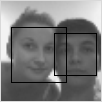
\includegraphics{opencv.png}
    \caption{Detekce obličejů v praxi}
\end{center}
\end{listing}

Algoritmus pro hledání obličejů je použit z knihovny OpenCV a tedy není záměrem
této kapitoly vysvětlovat jej. Byl pouze využit pro ukázku možností e-puck
knihovny.

\subsection{Zdrojový kód}

\begin{mylisting}
\begin{pyc}
#!/usr/bin/env python
# -*- coding: utf-8 -*-

import logging
import time

from Tkinter import *
from ImageTk import PhotoImage

import cv
import ImageDraw
import Image as Img

from epuck.controller import Controller

logging.basicConfig(level=logging.ERROR)

c = Controller('/dev/rfcomm0', timeout=5, asynchronous=True)

# Set camera properties
c.set_front_led(1)
c.set_camera(Controller.GREYSCALE_MODE, 55, 55, 8)

# Create the application layout
root = Tk()
img_face = Label(root)
img_face.pack()

# Load face definitions
cascade = cv.Load('haarcascade_frontalface_alt.xml')

def show_photo():
    # Get the photo
    img = c.get_photo() \
        .get_response() \
        .resize((100, 100), Img.ANTIALIAS)

    # Convert the photo for OpenCV
    cv_img = cv.CreateImageHeader(img.size, cv.IPL_DEPTH_8U, 1)
    cv.SetData(cv_img, img.tostring())

    # Find any faces in the image
    storage = cv.CreateMemStorage(0)
    cv.EqualizeHist(cv_img, cv_img)
    faces = cv.HaarDetectObjects(cv_img, 
                cascade, 
                storage, 
                1.2, 2,
                cv.CV_HAAR_DO_CANNY_PRUNING)

    if faces:
        for f in faces:
            # Draw a border around a found face.
            draw = ImageDraw.Draw(img)
            draw.setfill(0)
            draw.rectangle([(f[0][0],
                             f[0][1]),
                            (f[0][0] + f[0][2],
                             f[0][1] + f[0][3])])

    # Show the image with faces
    image = PhotoImage(img)
    img_face.config(image=image)
    img_face.img = image

    # Run this function again in 10ms
    img_face.after(10, show_photo)

# Get first photo and run the main loop
show_photo()
root.mainloop()
\end{pyc}
\captionof{listing}{Grafická aplikace pro detekci obličejů}
\label{opencv}
\end{mylisting}

\subsection{Vysvětlení programu}

Program se skládá z několika částí, které využívají jednotlivé knihovny, na
začátku (zdrojový kód \ref{kamera_okno}) je třeba nastavit kameru robota. Pro
detekci obličejů se používá černobilých fotek, takže bylo možné zvětšit
velikost fotografie. Dále je nutné vytvořit grafické okno pomocí knihovny
Tkinter a načíst data pro knihovnu OpenCV, která používá pro detekci obličejů.

\begin{listing}
\begin{pyc*}{firstnumber=20}
# Set camera properties
c.set_front_led(1)
c.set_camera(Controller.GREYSCALE_MODE, 55, 55, 8)

# Create the application layout
root = Tk()
img_face = Label(root)
img_face.pack()

# Load face definitions
cascade = cv.Load('haarcascade_frontalface_alt.xml')
\end{pyc*}
\caption{Nastavení kamery a vytvoření okna}
\label{kamera_okno}
\end{listing}

Hlavní část je ve funkci \code{show\_photo}, která je pravidelně volána hlavní
smyčkou knihovny Tkinter. V ní pak dochází k zpracování a zobrazení obrázku z
robota. Nejprve (zdrojový kód \ref{photo_resize}) je získána fotka, ta je
následně zvětšena pro lepší prohlížení.

\begin{listing}
\begin{pyc*}{firstnumber=32}
def show_photo():
    # Get the photo
    img = c.get_photo() \
        .get_response() \
        .resize((100, 100), Img.ANTIALIAS)
\end{pyc*}
\caption{Získání fotografie a její zvětšení}
\label{photo_resize}
\end{listing}

Výsledek je převeden do formátu obrázků pro OpenCV. Dále je zavolán algoritmus
pro detekci obličejů, nalezené obličeje jsou zakresleny do fotky (zdrojový kód
\ref{opencv_part}).

\begin{listing}
\begin{pyc*}{firstnumber=38}
    # Convert the photo for OpenCV
    cv_img = cv.CreateImageHeader(img.size, cv.IPL_DEPTH_8U, 1)
    cv.SetData(cv_img, img.tostring())

    # Find any faces in the image
    storage = cv.CreateMemStorage(0)
    cv.EqualizeHist(cv_img, cv_img)
    faces = cv.HaarDetectObjects(cv_img, 
                cascade, 
                storage, 
                1.2, 2,
                cv.CV_HAAR_DO_CANNY_PRUNING)

    if faces:
        for f in faces:
            # Draw a border around a found face.
            draw = ImageDraw.Draw(img)
            draw.setfill(0)
            draw.rectangle([(f[0][0],
                             f[0][1]),
                            (f[0][0] + f[0][2],
                             f[0][1] + f[0][3])])
\end{pyc*}
\caption{Zpracování fotky pomocí OpenCV}
\label{opencv_part}
\end{listing}

Nakonec už je fotka naposledy převedena, tentokrát do formátu pro Tkinter, a
zobrazena (\ref{tkinter_show}). Funkce \code{after} slouží k periodickému
volání metody \code{show\_photo} každých 10ms. Díky tomu by se měl obraz
aktualizovat téměř v reálném čase (samozřejmě je snímání fotky v robotovi
znatelné na časové prodlevě).

\begin{listing}
\begin{pyc*}{firstnumber=61}
    # Show the image with faces
    image = PhotoImage(img)
    img_face.config(image=image)
    img_face.img = image

    # Run this function again in 10ms
    img_face.after(10, show_photo)
\end{pyc*}
\caption{Převedení a zobrazeni fotky pomocí Tkinter}
\label{tkinter_show}
\end{listing}
%}}}
\chapter{Závěr} %{{{

    \section{Zhodnocení práce}

    Ve své práci jsem splnil všechny cíle, které jsem si vytyčil. Vznikla
    knihovna, která v sobě odráží základní myšlenku programovacího jazyka
    Python, ve kterém je napsána. Programování je intuitivní, lehce
    pochopitelné, je možné rychlé prototypování třeba jen části kódu, nebo
    interaktivní ovládání robota z interpretu. Na druhou stranu knihovna nabízí
    i podporu pro vytváření aplikací, kde se můžeme spolehnout, že každý
    zaslaný příkaz bude proveden.

    Uživatel dostává možnost si vybrat mezi transparentní synchronní
    komunikací, anebo asynchronní komunikací, u které nemusí čekat na přijetí
    odpovědi. Tady se jedná o velkou výhodu pro vytváření aplikací, které mohou
    pracovat s došlými daty, zatímco čekají na další, anebo jde pouze o
    interaktivitu aplikace, kde není přípustné, aby docházelo k prodlevám,
    zatímco program čeká na odpověď.

    Dalším úspěchem je přepracování firmware BTcom, napsaného v jazyku C a
    nahrávaného přímo do robota, který je standardně dodáván s e-puck robotem.
    Díky mým úpravám je možné velmi přesně párovat zaslané příkazy a došlé
    odpovědi. Dále jsem upravil binární odpovědi, aby začínaly hlavičkou
    obsahující informace o příkazu a velikost přenášených dat. Zpracování došlé
    binární odpovědi tak není závislé na hádání, ke kterému příkazu odpověď
    patří. Díky těmto změnám jsem mohl vytvořit kontrolní mechanismy
    zabraňující ztrátě příkazů. Každý příkaz má danou časovou lhůtu, do které
    musí dojít odpověď, jinak je považován za ztracený a odeslán znova.

    Pokusil jsem se i vyřešit některé základní problémy, které provázejí e-puck
    robota. Situaci, kdy robot přestává reagovat, protože mu dochází baterie,
    jsem vyřešil optickou signalizací. Jedná se na první pohled o drobnou
    změnu, ovšem pro programování robota jde o neocenitelnou pomůcku. Obzvlášť
    když si student robota půjčuje v počítačové laboratoři a tak si nikdy
    nemůže být jistý, kdy byl naposledy dobíjen.

    Pro uživatele knihoven neexistuje nic horšího, než když mají dokumentaci
    jednotlivých metod, ale nedočtou se jak tyto spojit dohromady a vytvořit
    tak ucelený program. Proto jsem jako součást práce napsal několik
    ukázkových programů, které ukazují jak snadné je knihovnu používat a
    integrovat s jinými knihovnami. Ovládání robota jde triviálně propojit s
    grafickým rozhraním pomocí knihovny Tkinter, s fotkami získanými z kamery
    robota jde pracovat pomocí Python Imaging Library (PIL) a díky tomu je
    možné použít libovolnou knihovnu pro práci s obrázky (např. OpenCV pro
    počítačové vidění).

    \section{Benchmark knihovny}

    Pro vzdálené ovládání robota je důležité jak rychle můžeme reagovat na
    podněty z prostředí. Vyzkoušíme si tedy některé základní příkazy a budeme
    stopovat jak rychle se provádějí.

    Nejprve začneme zjištěním údajů ze senzorů překážek. Kód \ref{time1} (pouze
    relevantní část) měří kolikrát za sekundu je možné získat údaje z IR
    senzorů. Program jsem nechal běžet 500 sekund. Nejlepší výsledek bylo 50
    zavolání příkazu, nejhorší výsledek bylo jen 30 zavolání příkazu, v průměru
    bylo posláno 39 příkazů. To je tedy v průměru 25ms na jednu iteraci.

\begin{listing}
\begin{pyc}
start_time = time.time()
count = [0]
while True:
    prox = c.get_proximity_sensors().get_response()
    count[-1] += 1
    if time.time() - start_time > 1:
        print count
        count.append(0)
        start_time = time.time()
\end{pyc}
\caption{Stopování rychlosti senzorů překážek}
\label{time1}
\end{listing}

    Zkusíme, jak moc se od sebe liší různé příkazy. V kódu \ref{time2} budeme
    získávat fotku z kamery. Pro barevné fotky s rozměry 40x40 je možné za
    sekundu v průměru získat 3 snímky. Tady musíme započítat i převod z módu
    RGB565 do formátu používaného knihovnou PIL. Pokud nám bude stačit pouze
    černobílý obrázek stejných rozměrů, tak za sekundu jsme schopni jich získat
    v průměru 5.

\begin{listing}
\begin{pyc}
start_time = time.time()
count = [0]
while True:
    c.get_photo().get_response()
    count[-1] += 1
    if time.time() - start_time > 1:
        print count
        count.append(0)
        start_time = time.time()
        \end{pyc}
\caption{Stopování rychlosti kamery}
\label{time2}
\end{listing}

    Stačilo nám tedy jen pár pokusů abychom zjistili, že možný počet zaslaných
    příkazů za sekundu se dramaticky liší v závislosti na typu příkazu anebo
    jeho parametrech. Důležité je také si uvědomit, že při asynchronní
    komunikaci po zavolání příkazu nemusíme čekat na odpověď a můžeme tedy
    ihned volat další příkaz. To s sebou nese jedno riziko, pokud budeme
    posílat nové příkazy rychleji, než je stíhá robot vykonávat, tak nám může
    přetéct fronta příkazů, která není nekonečná. Každé zavolání příkazu, který
    potřebuje načíst data nám tuto frontu vyprázdní, protože se vždy musejí
    provést všechny předchozí příkazy a teprve pak je možné získat data, ale i
    tak je dobrým zvykem omezit maximální rychlost smyčky programu krátkou
    pauzou.

%}}}
\appendix

\chapter{Dokumentace API}%{{{
\label{dokumentace api}

\section{Modul {\tt epuck}}

\subsection{Třída \code{Controller}}
class \code{epuck.{\bf Controller}(port[, asynchronous=False[, timeout=0.5[,\\
        max\_tries=10]]])}
    \begin{popis}
    Ovládání e-puck robota přes Bluetooth z počítače.

    Při vytváření objektu je možné rozhodnout, zda-li má komunikace probíhat
    synchronně, anebo asynchronně. Tato volba ovlivňuje zda-li se pro
    komunikaci použije třída \code{SyncComm} anebo \code{AsyncComm}. Také na této
    volbě závisí co budou jednotlivé příkazy vracet. V případě synchronní
    komunikace půjde rovnou o odpověď. V případě asynchronní komunikace vrátí
    \code{RequestHandler}. Z něj se stejné informace dají získat pomocí metody
    \code{get\_response()} (další podrobnosti v dokumentaci třídy
    \code{RequestHandler}).

    {\bf Poznámka: }V této dokumentaci jsou popsány návratové hodnoty tak, jak
    je vrátí přímo příkaz při synchronní komunikaci, anebo jak budou vráceny
    metodou \code{get\_response()} třídy \code{RequestHandler} při komunikaci
    asynchronní.

    {\bf Parametry: }
    \begin{itemize}
        \item {\bf port}(string) -- cesta k portu, kde je e-puck připojen
            (například \code{/dev/rfcomm2})
        \item {\bf asynchronous} (bool) -- zda-li má být použita asynchronní
            komunikace.
        \item {\bf timeout} (float) -- čas v sekundách před dalším pokusem o
            zaslání příkazu (asynchronní komunikace)
        \item {\bf max\_tries} (int) -- maximální počet pokusů o zaslání
            příkazu (asynchronní komunikace)
    \end{itemize}

    \method{{\bf set\_speed}(left, right)}
        \begin{popis}
        Nastavit rychlost levého a pravého krokového motoru. Rychlost je měřena
        v krocích za sekundu a musí být v rozmezí [-1000, 1000].

        Pokud je rychlost mimo rozsah, tak vyvolá výjimku \code{WrongCommand}.
        Při asynchronní komunikaci může dojít k vypršení limitu pokusů a pak
        dojde k vyvolání výjimky \code{CommError}.

        {\bf Parametry: }
        \begin{itemize}
            \item {\bf left} (int) -- požadovaná rychlost levého kola
            \item {\bf right} (int) -- požadovaná rychlost pravého kola
        \end{itemize}
        \end{popis}

    \method{{\bf get\_speed}()}
        \begin{popis}
        Získat rychlost levého a pravého krokového motoru. Rychlost je měřena v
        krocích za sekundu a je v rozmezí [-1000, 1000].

        {\bf Návratová hodnota: }dvojice obsahující rychlost levého a pravého
        motoru
        \end{popis}

    \method{{\bf set\_body\_led}(on)}
        \begin{popis}
        Zapnout nebo vypnout zelenou diodu v robotovi.

        {\bf Parametry: }
        \begin{itemize}
            \item {\bf on} (bool) -- zapnout nebo vypnout diodu
        \end{itemize}
        \end{popis}

    \method{{\bf set\_front\_led}(on)}
        \begin{popis}
        Zapnout nebo vypnout jasnou červenou diodu v přední části robota (vedle
        kamery).

        {\bf Parametry: }
        \begin{itemize}
            \item {\bf on} (bool) -- zapnout nebo vypnout diodu
        \end{itemize}
        \end{popis}

    \method{{\bf set\_leds}(on)}
        \begin{popis}
        Zapnout nebo vypnout všechny diody, které jsou po obvodu robota, naráz.

        {\bf Parametry: }
        \begin{itemize}
            \item {\bf on} (bool) -- zapnout nebo vypnout diody
        \end{itemize}
        \end{popis}

    \method{{\bf set\_led}(led\_no, on)}
        \begin{popis}
        Zapnout nebo vypnout jednu z osmi diod, které jsou po obvodu robota.

        Diody jsou očíslovány 0 až 7, po směru hodinových ručiček, dioda číslo
        0 je v přední části robot (neplést s jasnější diodou, která je vedle
        kamery).

        {\bf Parametry: }
        \begin{itemize}
            \item {\bf led\_no} (int) -- číslo diody, která má být ovládána
                (číslo z rozsahu [0, 7])
            \item {\bf on} (bool) -- zapnout nebo vypnout diodu
        \end{itemize}
        \end{popis}

    \method{{\bf get\_turning\_switch}()}
        \begin{popis}
        Získat pozici otáčivého přepínače.

        Otáčivý přepínač je na horní straně robota, jde o malou černou tyčinku,
        kterou je možné otočit do jedné z 16 pozic. Pozice jsou očíslovány 0 až
        15. Přepínač je v pozici 0 pokud šipka ukazuje směrem k černé tečce,
        která je nakreslená na plošném spoji. Pozice jsou číslovány ve směru
        hodinových ručiček.

        {\bf Návratová hodnota:} pozice přepínače.
        \end{popis}

    \method{{\bf get\_proximity\_sensors}()}
        \begin{popis}
            Získat data o vzdálenosti překážek z 8 IR senzorů.

            Senzory vrací hodnotu z rozsahu [0, 4095]. Jsou rozmístěny po
            obvodu robota zrcadlově na pravé i levé straně. Pokud bereme směr
            pohybu jako úhel 0 stupňů, tak se senzory nachází na 10, 45 a 90
            stupních a také jsou dva vlevo i vpravo na zadní části robota.

            Metoda vrací vždy hodnoty všech senzorů. Pro přehlednější
            zpracování jsou uloženy ve slovníku, klíč je vždy znak označující
            levou (L) nebo pravou (P) stranu a pak uhel v jakém se senzor
            nachází (senzory vzadu jsou označeny B). Seznam klíčů tedy je: {\tt
            ['R10', 'R45', 'R90', 'RB', 'LB', 'L90', 'L45', 'L10']}.

            {\bf Návratová hodnota:} hodnoty IR senzorů překážek.
        \end{popis}

    \method{{\bf get\_ambient\_sensors}()}
        \begin{popis}
        Získat data o okolním světle z 8 IR senzorů.

        Senzory vrací hodnotu z rozsahu [0, 4095]. Jsou rozmístěny po obvodu
        robota zrcadlově na pravé i levé straně. Pokud bereme směr pohybu jako
        úhel 0 stupňů, tak se senzory nachází na 10, 45 a 90 stupních a také
        jsou dva vlevo i vpravo na zadní části robota.

        Metoda vrací vždy hodnoty všech senzorů. Pro přehlednější zpracování
        jsou uloženy ve slovníku, klíč je vždy znak označující levou (L) nebo
        pravou (P) stranu a pak uhel v jakém se senzor nachází (senzory vzadu
        jsou označeny B). Seznam klíčů tedy je {\tt ['R10', 'R45', 'R90', 'RB',
        'LB', 'L90', 'L45', 'L10']}.

        {\bf Návratová hodnota:} naměřené hodnoty okolního světla.
        \end{popis}

    \method{{\bf set\_camera}(mode, height, width, zoom)}
        \begin{popis}
        Nastavit parametry kamery.

        E-puck obsahuje kameru o rozlišení 640x480, avšak není možné využít
        její plnou kapacitu z paměťových důvodů. Proto je třeba nastavit jak
        velký obrázek uživatel očekává a také jaké prokládání má být použito.
        Kamera je v robotovi umístěna otočená, ale uživatel dostane už obraz
        správně orotovaný. Je však dobré na tento fakt myslet při zadávání
        šířky a výšky. Pokud je zoom 2 nebo 4, tak se o prokládání stará přímo
        kamera a zrychlí se tak patřičně framerate.

        Například pro rozměry 40x40 a zoom 8 robot vezme ze senzorů kamery
        obdélník velikosti 320x320 a z něj každý 8. pixel.

        Na parametry jsou kladeny následující požadavky:
        \begin{itemize}
            \item velikost * zoom nesmí překročit kapacitu kamery,
            \item velikost dat je omezena velikostí bufferu, který je zhruba
                4kB a
            \item zoom by měl být z rychlostních důvodů mocninou dvojky.
        \end{itemize}

        Na formát fotografie nejsou kladena žádná další omezení, co se poměru
        stran týče. Je tedy možné získat i lineární obraz 480x1.

        Kamera může fotit v režimu rgb565 anebo v režimu stupňů šedi. Pro každý
        pixel pak používá buď 16 anebo 8 bitů. V režimu šedi je pak framerate
        dvojnásobný.

        {\bf Parametry:}
        \begin{itemize}
            \item {\bf mode} -- mód kamery, buď \code{Controller.RGB565\_MODE},
                anebo \\ \code{Controller.GREYSCALE\_MODE},
            \item {\bf width} (int) -- šířka požadované fotografie,
            \item {\bf height} (int) -- výška požadované fotografie,
            \item {\bf zoom} (int) -- velikost prokládání fotografie.
        \end{itemize}
        \end{popis}

    \method{{\bf get\_camera}()}
        \begin{popis}
        Získat nastavení kamery.

        Metoda vrací slovník s parametry odpovídajícími parametrům metody
        \code{set\_camera()}.

        {\bf Návratová hodnota:} slovník s nastavením kamery:
        \begin{itemize}
            \item {\bf mode} -- mód kamery, buď \code{Controller.RGB565\_MODE},
                anebo \\ \code{Controller.GREYSCALE\_MODE},
            \item {\bf width} (int) -- šířka požadované fotografie,
            \item {\bf height} (int) -- výška požadované fotografie,
            \item {\bf zoom} (int) -- velikost prokládání fotografie.
        \end{itemize}
        \end{popis}

    \method{{\bf get\_photo}()}
        \begin{popis}
        Získat fotku z kamery.

        Fotka je ve formátu, jaký byl zadán metodou \code{set\_camera()}. Pokud
        nebylo nastavení měněno, tak je získána barevná fotka 40x40 pixelů se
        zoomem 8.

        Pro ulehčení práce s fotkou je vrácena jako instance třídy \code{Image}
        z PIL (Python Imaging Library).

        {\bf Návratová hodnota:} Fotka z kamery (typu \code{Image})
        \end{popis}

    \method{{\bf reset}()}
        \begin{popis}
        Resetovat robota.

        Proběhne restart robota. Všechno nastavení se anuluje, robot se
        zastaví.
        \end{popis}

    \method{{\bf set\_motor\_pos}(left, right)}
        \begin{popis}
        Nastavení čítačů pro krokové motory.

        U obou krokových motorů je možné aktuálnímu pozici kola přiřadit číslo,
        to pak bude s každým krokem motoru inkrementováno nebo dekrementováno.
        Pozice se počítají jako 16bitové číslo se znaménkem.

        Počet vykonaných kroků je možné zjistit odečtením nastavených hodnot od
        hodnot získaných metodou \code{get\_motor\_pos()}.

        {\bf Parametry:}
        \begin{itemize}
            \item {\bf left} (int) -- nová hodnota čítače pro levý motor,
            \item {\bf right} (int) -- nová hodnota čítače pro levý motor.
        \end{itemize}
        \end{popis}

    \method{{\bf get\_motor\_pos}()}
        \begin{popis}
        Získat aktuální hodnotu čítačů krokových motorů.

        U obou krokových motorů je možné aktuálnímu pozici kola přiřadit číslo
        pomocí metody \code{set\_motor\_pos()}, to pak bude s každým krokem
        motoru inkrementováno nebo dekrementováno. Pozice se počítají jako
        16bitové číslo se znaménkem.

        {\bf Návratová hodnota:} dvojice hodnot čítačů (levý motor, pravý
        motor).
        \end{popis}

    \method{{\bf get\_raw\_accelerometer}()}
        \begin{popis}
        Získat vektor akcelerace.

        Vektor se skládá ze složek x, y a z. Vrácená data jsou uložena ve
        slovníku, klíčem je vždy směr ("x", "y" nebo "z"). Pro získání
        praktičtějších dat viz \code{get\_accelerometer()}.

        {\bf Návratová hodnota:} slovník se třemi složkami vektoru akcelerace
        (klíče jsou "x", "y" a "z")
        \end{popis}

    \method{{\bf get\_accelerometer}()}
        \begin{popis}
        Získat data z akcelerometru ve sférických souřadnicích.

        Robot z vektoru akcelerometru vypočítá tři veličiny, s kterými se lépe
        pracuje. Jsou jimi zrychlení, náklon a orientace. Všechny tři jsou
        vyjádřeny ve stupních. Jejich význam je následující:

        \begin{description}
            \item[Akcelerace] \hfill\\ Velikost vektoru = intenzita zrychlení.
            \item[Náklon] \hfill \\ \vspace{-5mm}
                \begin{itemize}
                    \item 0$^{\circ}$ -- e-puck je horizontálně
                    \item 90$^{\circ}$ -- e-puck je vertikálně
                    \item 180$^{\circ}$ -- e-puck je horizontálně, ale vzhůru
                    nohama
                \end{itemize}
            \item[Orientace] -- odklon vektoru od horizontální roviny,
            0$^{\circ}$ míří dopředu \\ \vspace{-5mm}
            \begin{itemize}
                \item 0$^{\circ}$ -- přední část níže než zadní
                \item 90$^{\circ}$ -- levá část níže než pravá
                \item 180$^{\circ}$ -- zadní část níže než přední
                \item 270$^{\circ}$ -- pravá část níže než levá
            \end{itemize}
        \end{description}

        {\bf Poznámka:} Uvedené hodnoty veličin byly získány z dokumentace
        knihovny pro firmware e-puck robota. Při testech ne vždy odpovídaly
        realitě, proto je důležité si důkladně vyzkoušet jaké hodnoty robot
        vykazuje při různých činnostech a vytvořit si vlastní závěry.

        {\bf Návratová hodnota:} slovník se třemi veličinami získanými z
        vektoru akcelerace. Klíče jsou:
        \begin{itemize}
            \item {\bf acceleration} -- akcelerace
            \item {\bf inclination} -- náklon
            \item {\bf orientation} -- orientace
        \end{itemize}
        \end{popis}

    \method{{\bf calibrate\_sensors}()}
        \begin{popis}
        Kalibrace IR senzorů.

        Pro kalibraci IR senzorů je nutné přesvědčit se, že v dosahu senzorů
        není žádná překážka. Kalibrace probíhá vždy po zapnutí robota, tedy
        není nutné ji pouštět manuálně, pouze pokud by senzory vykazovaly
        nějaké závažnější odchylky v naměřených hodnotách.
        \end{popis}

    \method{{\bf stop}()}
        \begin{popis}
        Zastavit robota.

        Dojde k zastavení motorů robota a k vypnutí všech LED.
        \end{popis}

    \method{{\bf play\_sound}(sound\_no)}
        \begin{popis}
        Přehrát zvuk.

        V robotovi je uloženo 5 zvuků ve formátu wav. Parametr sound\_no
        označuje číslo zvuku, který se má přehrát:

        \begin{enumerate}
            \item "haa"
            \item "spaah"
            \item "ouah"
            \item "yaouh"
            \item "wouaaaaaaaah"
        \end{enumerate}

        Dle názvů je jasné o jaké zvuky se jedná. Jde o citoslovce výkřiků
        (robot má většinou tendence narážet do věcí okolo sebe). Pokud bude
        zadáno jiné číslo, tak dojde k vypnutí speakeru. Tím pádem také
        přestane šum, který zůstane hrát po přehraném zvuku.

        {\bf Parametry:}
        \begin{itemize}
            \item {\bf sound\_no} (int) -- číslo označující zvuk, který se má
            přehrát
        \end{itemize}
        \end{popis}

    \method{{\bf get\_volume}()}
        \begin{popis}
        Získat úrovně hlasitosti z mikrofonů.

        Robot disponuje třemi mikrofony rozmístěnými na horní straně. Jsou
        rozmístěny vlevo, vpravo a vzadu. Protože samotná nahraná data jsou
        příliš velká, tak robot dokáže pouze poslat úroveň hlasitosti zvuků
        snímaných jednotlivými mikrofony.

        Data jsou vrácena jako slovník, jednotlivé mikrofony jsou označeny
        zkratkou jejich umístění ("R", "L", "B").

        {\bf Návratová hodnota:} úroveň hlasitosti na jednotlivých mikrofonech,
        klíče jsou \code{["R", "L", "B"]}.
        \end{popis}

    \method{{\bf get\_microphone}(on)}
        \begin{popis}
        Získání hodnot z mikrofonu.

        Začne načítání dat z mikrofonu. Tato data pak budou převedena v
        robotovi pomocí FFT a zaslána do počítače. Jakmile je jednou zapnuto
        nahrávání, tak každý následující příkaz si už jen vyzvedne připravená
        data.

        Data jsou vrácena jako seznam komplexních čísel.

        {\bf Parametry:}
        \begin{itemize}
            \item {\bf on} (int) -- zapnout / vypnout nahrávání dat z mikrofonu
        \end{itemize}

        {\bf Návratová hodnota:} seznam dat získaných z FFT
        \end{popis}
    \end{popis}

\subsection{Výjimky}

\noindent exception \code{epuck.{\bf EPuckError}}
    \begin{popis}
    Základní výjimka v modulu \code{epuck}. Všechny ostatní od ní dědí.
    \end{popis}

\vskip5mm
\noindent exception \code{epuck.{\bf ControllerError}}
    \begin{popis}
    Chyba při práci s robotem. Například se nepovedlo k robotovi vůbec
    připojit.
    \end{popis}

\vskip5mm
\noindent exception \code{epuck.{\bf WrongCommand}}
    \begin{popis}
    Specializace výjimky ControllerError. Uživatel nejspíše zadal špatný
    příkaz, např. parametry, které jsou mimo povolené rozsahy.
    \end{popis}

\section{Modul {\tt epuck.comm}}
Při komunikaci s robotem si uživatel může vybrat mezi synchronní anebo
asynchronní komunikací. Rozhodnutí uživatele při vytváření instance třídy
\code{Controller} rozhodne o tom, zda-li se pro komunikaci s robotem využije
třída \code{SyncComm} anebo \code{AsyncComm}. Přesný popis těchto tříd je k
nalezení v programátorské dokumentaci, uživatel je využívá pouze
prostřednictvím třídy \code{Controller}.

Důležité je ovšem vědět jaké výjimky můžou vzniknout při komunikaci s robotem.
Všechny výjimky samozřejmě dědí od \code{EPuckError}. Obecně pro chybu při
komunikaci slouží výjimka \code{CommError}. Od ní pak dědí výjimky pro
jednotlivé druhy komunikace: \code{SyncCommError} a \code{AsyncCommError}.

Další důležitý rozdíl mezi sériovou a asynchronní komunikací je ve vrácené
hodnotě z metod třídy \code{Controller}. Pro synchronní komunikaci jsou vrácena
přímo odpověď. Pro asynchronní komunikaci je ovšem vrácen pouze instance třídy
\code{RequestHandler}, pomocí kterého uživatel může zjistit zda-li už byla
přijata odpověď a posléze ji získat.

\subsection{Odpověď u asynchronní komunikace}
class \code{epuck.comm.{\bf RequestHandler}}
\begin{popis}
    Jedná se o objekt reprezentující odpověď na příkaz zaslaný robotovi při
    asynchronní komunikaci. U asynchronní komunikace je důležité, aby poslání
    příkazu nezablokovalo vlákno, v kterém byl příkaz poslán. Proto není možné
    čekat na odpověď. Uživatel ovšem nezůstane bez odpovědi. Příkaz mu vrátí
    právě tento handler, pomocí kterého dokáže zjistit, zda-li už odpověď došla
    a případně i získat onu odpověď.

    \method{{\bf response\_received}()}
        \begin{popis}
        Slouží ke kontrole, zda-li už došla odpověď od robota. Neblokuje vlákno
        a nevrací odpověď. K jejímu získání slouží metoda
        \code{get\_response()}.

        {\bf Návratová hodnota: } informace, zda-li už došla odpověď.
        \end{popis}

    \method{{\bf get\_response}()}
        \begin{popis}
        Zkontroluje, zda-li došla odpověď, pokud ano, tak ji vrátí, v opačném
        případě počká dokud nedorazí a pak ji vrátí. Z toho důvodu zablokuje
        vlákno, pokud ještě odpověď nedošla.

        Pokud je možné pokračovat ve vykonávání program bez této odpovědi, tak
        se doporučuje nejprve kontrolovat přítomnost odpovědi pomocí metody
        \code{response\_received()}.

        {\bf Návratová hodnota: } odpověď od robota, přesný druh odpovědi k
        nalezení v dokumentaci třídy \code{Controller}.
        \end{popis}

    \method{{\bf error\_raised}()}
        \begin{popis}
        Kontrola, zda-li při vykonání příkazu nevznikla výjimka.

        Výjimka je uložena v atributu \code{error}. Bude vyhozena pokud se
        uživatel pokusí přistoupit k odpovědi, anebo zavolá metodu
        \code{join}.

        {\bf Návratová hodnota:} byla vyhozena výjimka.
        \end{popis}

    \method{{\bf join}()}
        \begin{popis}
        Vyčkání na provedení příkazu.

        Zablokuje vykonávání programu dokud nepřijde odpověď na příkaz.
        \end{popis}
\end{popis}

\subsection{Výjimky}

exception \code{epuck.comm.{\bf CommError}}
\begin{popis}
Chyba při komunikaci s robotem. Nejčastější příčinou je, že robot neodpovídá.
\end{popis}

\vskip5mm \noindent exception \code{epuck.comm.{\bf SyncCommError}}
\begin{popis}
Chyba při synchronní komunikaci s robotem.
\end{popis}

\vskip5mm \noindent exception \code{epuck.comm.{\bf AsyncCommError}}
\begin{popis}
Chyba při asynchronní komunikaci s robotem.
\end{popis}




%}}}
%{{{ Seznam literatury
%%%
%%% Literatura se řadí abecedně. Úvádí se pouze literatura, na kterou se v textu odkazuje.
%%% Při odkazu na knihu se vždy uvádějí čísla stránek.

\bibliographystyle{czechiso}
\bibliography{literatura}

%}}}
\end{document}
